%% -----------------------------------------------------------
%% Projeto 1 da disciplina de INF2608 - Fundamentos de Computacao Grafica
%% Versao em LaTeX do relatorio tecnico-cientifico do ray tracer educacional.
% chktex-file 3
% chktex-file 13
% chktex-file 24
% chktex-file 36

\documentclass[portuguese]{sbcreviews-2025}%
\usepackage[misc,geometry]{ifsym} 

%\usepackage{graphicx} % carregada dentro da classe
%\usepackage{fontspec} % carregada dentro da classe
%\usepackage{fontawesome} % carregada dentro da classe
%\usepackage{color} % carregada dentro da classe
%\usepackage{hyperref} % carregada dentro da classe

\usepackage{aas_macros}
\usepackage[bottom]{footmisc}

\usepackage{tabularray}
% O pacote tabularray torna o uso dos pacotes abaixo desnecessarios.
%\usepackage{supertabular}
%\usepackage{multicol}
%\usepackage{multirow}

\usepackage{afterpage}
\usepackage{url}
\usepackage{pifont}

\setcitestyle{square}
\newcommand{\slidescite}[2]{\citep[pp.~#2]{#1}}
\newcommand{\pbrtcontentsurl}{https://pbr-book.org/4ed/contents.html}
\newcommand{\DeclarePBRTSectionURL}[2]{\expandafter\def\csname pbrturl@#1\endcsname{#2}}
\newcommand{\pbrtsectionurl}[1]{%
    \ifcsdef{pbrturl@#1}{\csname pbrturl@#1\endcsname}{\pbrtcontentsurl}%
}
\DeclarePBRTSectionURL{1.2}{https://pbr-book.org/4ed/Introduction/Photorealistic_Rendering_and_the_Ray-Tracing_Algorithm.html}
\DeclarePBRTSectionURL{3.5}{https://pbr-book.org/4ed/Geometry_and_Transformations/Normals.html}
\DeclarePBRTSectionURL{3.7}{https://pbr-book.org/4ed/Geometry_and_Transformations/Bounding_Boxes.html}
\DeclarePBRTSectionURL{5.2}{https://pbr-book.org/4ed/Cameras_and_Film/Projective_Camera_Models.html}
\DeclarePBRTSectionURL{7.3}{https://pbr-book.org/4ed/Primitives_and_Intersection_Acceleration/Bounding_Volume_Hierarchies.html}
\DeclarePBRTSectionURL{8.1}{https://pbr-book.org/4ed/Sampling_and_Reconstruction/Sampling_Theory.html}
\DeclarePBRTSectionURL{8.5}{https://pbr-book.org/4ed/Sampling_and_Reconstruction/Stratified_Sampler.html}
\DeclarePBRTSectionURL{9.3}{https://pbr-book.org/4ed/Reflection_Models/Specular_Reflection_and_Transmission.html}
\DeclarePBRTSectionURL{9.5}{https://pbr-book.org/4ed/Reflection_Models/Dielectric_BSDF.html}
\DeclarePBRTSectionURL{11.2}{https://pbr-book.org/4ed/Volume_Scattering/Transmittance.html}
\DeclarePBRTSectionURL{12.4}{https://pbr-book.org/4ed/Light_Sources/Area_Lights.html}
\newcommand{\pbrtbook}{\emph{Physically Based Rendering} (PBRT 4e)}
\newcommand{\pbrtsec}[1]{\citep[\href{\pbrtsectionurl{#1}}{Se\c{c}\~ao~#1}]{pharr2023pbrt}}
\newcommand{\pbrtsecs}[1]{\citep[\href{\pbrtcontentsurl}{Se\c{c}\~oes~#1}]{pharr2023pbrt}}
\newcommand{\traceability}[1]{%
    \begin{quote}
    \footnotesize\textbf{Rastreabilidade no c\'odigo.}~#1
    \end{quote}
}

\definecolor{engtitle}{rgb}{0.5,0.5,0.5}
\definecolor{orcidlogo}{rgb}{0.37,0.48,0.13}
\definecolor{unilogo}{rgb}{0.16, 0.26, 0.58}
\definecolor{maillogo}{rgb}{0.58, 0.16, 0.26}
\definecolor{darkblue}{rgb}{0.0,0.0,0.0}
\hypersetup{colorlinks,breaklinks,
            linkcolor=darkblue,urlcolor=darkblue,
            anchorcolor=darkblue,citecolor=darkblue}
\emergencystretch=3em
\sloppy
\hbadness=10000
\vbadness=10000
\hfuzz=70pt
\vfuzz=2pt
\raggedbottom
%\hypersetup{colorlinks,citecolor=blue,linkcolor=blue,urlcolor=blue}
% We disable hyperlinks by default with this line, to avoid the error "\pdfendlink ended up in different nesting level" while writing.

\category{Projeto 1 da disciplina de INF2608 --\\Fundamentos de Computação Gráfica}
\title[Análise Técnico-Científica de Ray Tracing]{Análise Técnico-Científica\\de uma Implementação de Ray Tracing}
\engtitle{\textcolor{engtitle}{Technical-Scientific Analysis\\of a Ray Tracing Implementation}}

\author[Yang Ricardo Barcellos Miranda]{
\affil{\textbf{Yang Ricardo Barcellos Miranda}~[\href{mailto:ymiranda@inf.puc-rio.br}{\nolinkurl{ymiranda@inf.puc-rio.br}}]}
}

\institution{Pontifícia Universidade Católica do Rio de Janeiro - PUC-Rio}

\begin{document}

\hfuzz=70pt

\begin{frontmatter}

\maketitle

\begin{abstract-pt}
Este artigo apresenta uma análise técnico-científica de uma implementação de ray tracing desenvolvida no Projeto 1 da disciplina de INF2608. O objetivo é verificar, a partir do código efetivamente executável, quais componentes geométricos, fotométricos e amostrais foram materializados, como eles se relacionam com os materiais da disciplina e em que medida a implementação se aproxima das referências selecionadas de PBRT 4e. A análise evidencia um núcleo sólido de câmera pinhole, raio paramétrico, interseções analíticas, sombreamento local de Phong e sombras diretas, além de extensões como supersampling, instanciação afim, luz de área, reflexão com Fresnel-Schlick, refração com Lei de Snell, reflexão interna total, Beer-Lambert e transmitância acumulada em raios de sombra. Para triângulos e aceleração, o artigo distingue cuidadosamente entre o conteúdo teórico e o que está implementado: há suporte a \texttt{Triangle}, \texttt{TriangleMesh} e uma BVH estática local para malhas, mas não há um acelerador global de cena. O trabalho também discute a infraestrutura experimental do projeto, com CLI padronizada, persistência de artefatos de render e diagramas que reforçam a rastreabilidade entre formulação teórica, estrutura algorítmica e evidência visual.
\end{abstract-pt}

\begin{abstract-en}
This paper presents a technical-scientific analysis of a ray tracing implementation developed for the first INF2608 course project. Its main goal is to verify, from the executable code itself, which geometric, photometric, and sampling components were effectively implemented, how they relate to the course material, and to what extent the result aligns with selected PBRT 4e references. The analysis shows a solid core built around a pinhole camera, parametric rays, analytic intersections, local Phong shading, and direct shadows, as well as extensions such as supersampling, affine instancing, area lights, Fresnel-Schlick reflection, dielectric refraction with Snell's law, total internal reflection, Beer-Lambert attenuation, and accumulated transmittance for shadow rays. For triangles and acceleration, the paper carefully distinguishes between theoretical coverage and implemented functionality: the codebase supports \texttt{Triangle}, \texttt{TriangleMesh}, and a static local BVH for meshes, but not a global scene accelerator. The article also discusses the project's experimental infrastructure, including a standardized CLI, persistent render artifacts, and diagrams that strengthen the traceability between theoretical formulation, algorithmic structure, and visual evidence.
\end{abstract-en}

\begin{pchaves}
traçado de raios, computação gráfica, PBRT, BVH, amostragem, renderização fisicamente inspirada
\end{pchaves}

\begin{keywords}
ray tracing, computer graphics, PBRT, BVH, sampling, physically inspired rendering
\end{keywords}

\begin{dates}
\noindent{\sffamily\textbf{Entrega:}} 10/05/2026
\end{dates}

\end{frontmatter}
\section{Introdução}
\label{sec:escopo}

Este artigo apresenta uma análise técnico-científica da implementação de ray tracing disponível no repositório do Projeto 1~\citep{inf2608projectrepo}. O objeto principal da análise é o código em \path{src/ray_tracing_2/}, confrontado com os tópicos dos slides da disciplina, de autoria de Waldemar Celes (W.~Celes, \href{mailto:celes@inf.puc-rio.br}{celes@inf.puc-rio.br})~\citep{inf2608slides04,inf2608slides05,inf2608slides06}, e com referências selecionadas de \pbrtbook, em especial \pbrtsecs{1.2, 3.5, 3.7, 5.2, 7.3, 8.1, 8.5, 9.3, 9.5, 11.2 e 12.4}.

O objetivo não é recontar genericamente o que um ray tracer deveria fazer, mas verificar o que esta implementação entrega de forma observável, quais decisões algorítmicas sustentam cada efeito visual e em que pontos o projeto simplifica ou parcializa o conteúdo teórico. A leitura adotada separa três camadas: a formulação geométrica e física discutida em aula, a tradução algorítmica efetivamente materializada no repositório e as lacunas entre a teoria de referência e o escopo implementado.

Ao longo do texto, os slides da disciplina, o PBRT 4e e o repositório aparecem como referências formais. Já a rastreabilidade interna do código é apresentada por caminho relativo, símbolo e linha, de modo a permitir inspeção local das decisões relevantes sem confundir documentação bibliográfica com evidência de implementação.

A organização da análise segue quatro frentes complementares:

\begin{enumerate}
    \item reconstituir o núcleo geométrico e fotométrico do traçador, com raio paramétrico, interseções, câmera pinhole, Phong e sombras;
    \item examinar as extensões ópticas e amostrais, incluindo supersampling, instanciação, luz de área, reflexão, refração e transmitância;
    \item avaliar a geometria triangular e a aceleração local por BVH, distinguindo implementação real de cobertura apenas teórica;
    \item consolidar experimentos breves, limitações atuais, diagramas de apoio e uma avaliação final do que a implementação entrega.
\end{enumerate}

Como fonte externa, foi usado apenas o conteúdo de \pbrtbook, com ênfase em câmera projetiva, teoria de amostragem, reflexão e transmissão especular, transmitância, luzes de área, caixas envolventes e BVHs. A edição consultada foi a quarta edição online dessa obra~\citep{pharr2023pbrt}.

\section{Núcleo Geométrico e Fotométrico do Traçador}
\label{sec:slide4}

\subsection{Conceitos Estruturantes do Núcleo de Referência}
\label{sec:slide4-conceitos}

O material introdutório de traçado de raios~\citep{inf2608slides04} organiza-se em torno de um conjunto pequeno de conceitos que estrutura todo o traçador de raios.

\begin{enumerate}
    \item \textbf{Raio paramétrico e visibilidade (pp. 7-9).} A formulação $\mathbf{r}(t)=\mathbf{o}+t\,\hat{\mathbf{d}}$ reduz a linha de visada a uma reta orientada; $t$ funciona como distância assinada ou paramétrica ao longo do feixe, e a visibilidade do ponto observado é determinada pelo menor $t>0$ compatível com uma superfície.
    \item \textbf{Interseções analíticas e controle numérico (pp. 10-18).} O plano é descrito por $(\mathbf{x}-\mathbf{p}_0)\cdot\hat{\mathbf{n}}=0$, enquanto a esfera leva à quadrática $at^2+bt+c=0$, cujo discriminante $\Delta$ classifica ausência, tangência ou dupla interseção; do ponto de vista computacional, essa geometria analítica só é robusta quando acompanhada por um critério de tolerância $\varepsilon$ para rejeitar paralelismos numéricos e auto-interseções.
    \item \textbf{Câmera pinhole, filme e mudança de base (pp. 19-39).} A câmera é construída por uma base ortonormal $(\hat{\mathbf{u}},\hat{\mathbf{v}},\hat{\mathbf{w}})$ e pela geometria do filme, com $\Delta v = f\tan(\theta/2)$ e $\Delta u = \Delta v\,(w/h)$; em síntese, esse bloco combina geometria projetiva com mudança de base entre espaço da câmera e espaço global.
    \item \textbf{Iluminação local e fotometria simplificada (pp. 40-43).} O modelo local de Phong combina a componente difusa lambertiana $\max(0,\hat{\mathbf{n}}\cdot\hat{\mathbf{l}})$ com a componente especular $\max(0,\hat{\mathbf{r}}\cdot\hat{\mathbf{v}})^s$; fisicamente, trata-se de um modelo local e fenomenológico, útil para capturar dependência angular sem resolver transporte global de luz.
    \item \textbf{Organização algorítmica da cena, sombras e luz ambiente (pp. 44-55).} O pipeline de \emph{closest hit} seleciona a primeira interseção visível, o raio de sombra transforma a iluminação direta em um teste de visibilidade até a fonte, e o termo ambiente $m_{amb}\,l_{amb}$ fecha o modelo como aproximação empírica da iluminação indireta ausente.
\end{enumerate}

Esses conceitos explicam por que as subseções seguintes podem ser lidas como desdobramentos detalhados do mesmo núcleo conceitual.

\subsection{Raio paramétrico, visibilidade e registro de interseção}
\label{sec:slide4-raio}

O ponto de partida do Slide 4 é a modelagem do raio por

\[
\mathbf{r}(t)=\mathbf{o}+t\,\hat{\mathbf{d}},\qquad t\ge 0,
\]

em que $\mathbf{o}$ é a origem, $\hat{\mathbf{d}}$ é a direção normalizada e $t$ parametriza a posição ao longo do feixe. Em ótica geométrica, essa formulação abstrai a propagação retilínea da luz em meios homogêneos; em computação gráfica, ela converte o problema de visibilidade em um problema de encontrar o menor $t$ positivo compatível com uma superfície. Nos slides, isso aparece como o elo entre câmera, interseção e sombreamento local, particularmente na dedução do raio paramétrico e na interpretação física de $t$ como distância assinada ao longo da trajetória~\slidescite{inf2608slides04}{7--9}.

O repositório segue exatamente essa organização. O raio é carregado por \texttt{Ray}, enquanto \texttt{Hit} armazena a melhor interseção conhecida até o momento e também codifica \texttt{front\_face} e \texttt{backfacing}. Essa distinção, que no Slide 4 serve para consistência geométrica da normal, torna-se decisiva no Slide 5 para distinguir entrada e saída de meios refrativos. A rotina \texttt{Scene.compute\_intersection()} preserva o padrão clássico de \emph{closest hit}: percorre os objetos, atualiza um único registro acumulador e retorna apenas a interseção frontal mais próxima.

\traceability{\path{src/ray_tracing_2/hit.py} (\texttt{Hit}, l. 11; \texttt{set\_face\_normal()}, l. 25), \path{src/ray_tracing_2/scene.py} (\texttt{compute\_intersection()}, l. 24; \texttt{trace\_ray()}, l. 102).}

Ver também \pbrtsecs{1.2 e 3.5}.

\subsection[Interseções básicas: plano, esfera e controle numérico de epsilon]{Interseções básicas: plano, esfera e controle numérico de $\varepsilon$}
\label{sec:slide4-intersecoes}

Nos slides, o plano é descrito pela equação implícita

\[
(\mathbf{x}-\mathbf{p}_0)\cdot\hat{\mathbf{n}}=0,
\]

e a substituição de $\mathbf{r}(t)$ produz a solução linear

\[
t=\frac{(\mathbf{p}_0-\mathbf{o})\cdot\hat{\mathbf{n}}}{\hat{\mathbf{d}}\cdot\hat{\mathbf{n}}},
\]

exatamente como discutido nas páginas de interseção raio-plano~\slidescite{inf2608slides04}{10--13}. A esfera, por sua vez, impõe

\[
\lVert\mathbf{x}-\mathbf{c}\rVert^2-r^2=0,
\]

que, após substituição do raio, gera uma quadrática $at^2+bt+c=0$ cujo discriminante $\Delta=b^2-4ac$ decide ausência, tangência ou dupla interseção~\slidescite{inf2608slides04}{14--18}. Em ambos os casos, o aspecto fisicamente relevante é o mesmo: o que interessa para a câmera é a menor raiz positiva. O aspecto numericamente relevante também é comum: deve-se rejeitar soluções com $t$ demasiado pequeno para evitar reinterseção artificial da própria superfície.

O código espelha esse raciocínio. \texttt{Plane.intersect()} resolve o plano por produto escalar; \texttt{Sphere.intersect()} resolve a quadrática e guarda a menor raiz positiva; \texttt{Scene.offset\_point()} empurra a origem dos raios secundários ao longo da normal geométrica com \texttt{ray\_epsilon = 0.001}, evitando \emph{shadow acne} em sombra, reflexão e refração. O Slide 4 apresenta essa ideia como tolerância numérica; o repositório a aplica de forma centralizada, o que é arquiteturalmente melhor do que espalhar pequenos limiares por todos os materiais.

\traceability{\path{src/ray_tracing_2/shape.py} (\texttt{Sphere}, l. 17; \texttt{Sphere.intersect()}, l. 23; \texttt{Plane}, l. 54; \texttt{Plane.intersect()}, l. 60), \path{src/ray_tracing_2/scene.py} (\texttt{offset\_point()}, l. 33).}

Ver também \pbrtsec{1.2}.

\subsection{Câmera pinhole, filme e espaços de coordenadas}
\label{sec:slide4-camera}

O Slide 4 reconstrói o modelo pinhole por uma base ortonormal de câmera, usando \texttt{eye}, \texttt{center} e \texttt{up} para montar os eixos locais (pp. 19--23), e em seguida projeta amostras do pixel sobre o plano de imagem (pp. 24--29), antes de explicitar a mudança entre espaço de câmera e espaço global (pp. 31--39)~\citep{inf2608slides04}. A formulação algébrica é a de uma mudança de base: do espaço local da câmera para o espaço global da cena. Em uma formulação clássica, isso aparece como matriz de visualização, sua inversa e projeção perspectiva parametrizada por campo de visão, aspecto e distância ao plano de imagem.

No código, a ideia é a mesma, mas a implementação é condensada: \texttt{Camera.\_\_init\_\_()} usa \texttt{glm.lookAt()} para obter a transformação de visualização e armazena sua inversa em \texttt{inv\_view}. A geração do raio em \texttt{generate\_ray()} monta o ponto do pixel em espaço de câmera a partir de coordenadas normalizadas e da relação trigonométrica

\[
\Delta v = f\tan\left(\frac{\theta}{2}\right),\qquad \Delta u = \Delta v\,\frac{w}{h},
\]

que é precisamente a síntese entre geometria projetiva e semelhança de triângulos apresentada nos slides (pp. 24--29) e depois transforma esse ponto para o espaço global (pp. 31--39)~\citep{inf2608slides04}. O comentário recém-ajustado em \texttt{camera.py} deixa explícita uma nuance importante: \texttt{focal\_distance} aqui é distância geométrica ao plano de projeção no modelo pinhole, não distância focal de lente fina nem parâmetro de profundidade de campo. Esse detalhe é essencial para não projetar sobre o código uma física que ele não implementa.

Essa distinção também define uma limitação importante do projeto: todos os raios primários partem de um único centro ótico, sem abertura finita, círculo de confusão ou profundidade de campo. Portanto, o antialiasing implementado depois no Slide 5 altera a estratégia de amostragem do pixel, mas não muda o modelo óptico de formação de imagem.

Em \texttt{film.py}, \texttt{get\_sample()} e \texttt{render()} deixam claro que a imagem final é construída como média de amostras por pixel. Mesmo quando o caso básico usa apenas uma amostra central, a interface já está preparada para supersampling estocástico.

\traceability{\path{src/ray_tracing_2/camera.py} (\texttt{Camera}, l. 6; \texttt{\_\_init\_\_()}, l. 7; \texttt{generate\_ray()}, l. 23), \path{src/ray_tracing_2/film.py} (\texttt{Film}, l. 20; \texttt{get\_sample()}, l. 54; \texttt{render()}, l. 108), \path{src/ray_tracing_2/main.py} (\texttt{render()}, l. 25).}

Ver também \pbrtsec{5.2}.

\subsection{Phong, luz pontual, termo ambiente e sombra dura}
\label{sec:slide4-phong}

O Slide 4 fecha o núcleo do renderizador com o modelo local de Phong, isto é, uma soma de termo ambiente, componente difusa lambertiana e componente especular dependente do vetor refletido~\slidescite{inf2608slides04}{40--43, 54--55}. Em termos físicos, esse modelo não é um BRDF rigoroso, mas é uma aproximação útil: o termo difuso usa o fator $\max(0,\hat{\mathbf{n}}\cdot\hat{\mathbf{l}})$; o termo especular usa um pico angular em função de $\max(0,\hat{\mathbf{r}}\cdot\hat{\mathbf{v}})^s$; a sombra dura decorre de um teste binário de visibilidade entre o ponto sombreado e a fonte~\slidescite{inf2608slides04}{51--53}. Em particular, as páginas 40--43 articulam a síntese física mínima do projeto: incidência luminosa, orientação local de normal e dependência angular da resposta da superfície.

\texttt{PhongMaterial.direct\_lighting()} implementa exatamente esse cálculo. Para cada luz, o código obtém radiância incidente e direção via \texttt{sample\_radiance()}, soma o termo difuso e depois o termo especular. \texttt{Scene.transmittance()} faz o papel do raio de sombra, mas já em uma forma mais geral: para meios opacos, ele reduz-se ao teste binário do Slide 4; para meios transparentes, ele vira um produto acumulado de transmitâncias, o que antecipa o Slide 5.

Há, contudo, uma nuance importante entre a física dos slides e a convenção da implementação: os slides apresentam a lei usual de decaimento geométrico de uma fonte pontual, proporcional a $1/r^2$, mas \texttt{PointLight.radiance()} não aplica esse fator. O comentário do código explicita a razão: o projeto preserva a convenção do enunciado em que \texttt{power} é tratado como radiância constante da fonte. Isso não é um erro, mas uma simplificação de modelagem que precisa ser declarada no relatório para evitar falsa equivalência com uma formulação radiométrica completa.

\traceability{\path{src/ray_tracing_2/light.py} (\texttt{PointLight}, l. 42; \texttt{PointLight.radiance()}, l. 46), \path{src/ray_tracing_2/material.py} (\texttt{PhongMaterial}, l. 37; \texttt{direct\_lighting()}, l. 45; \texttt{eval()}, l. 72), \path{src/ray_tracing_2/scene.py} (\texttt{transmittance()}, l. 48), \path{src/ray_tracing_2/main.py} (\texttt{Sphere}, l. 54; \texttt{Plane}, l. 55; \texttt{PointLight}, l. 59).}

Ver também \pbrtsec{1.2}.

A síntese consolidada de aderência entre o núcleo geométrico-fotométrico de referência e a implementação atual foi deslocada para a Seção~\ref{sec:quadros-aderencia}, de modo a preservar a continuidade argumentativa desta parte analítica.
  
\section{Extensões Ópticas, Amostrais e de Transformação}
\label{sec:slide5}

\subsection{Antialiasing como integração estocástica sobre o pixel}
\label{sec:slide5-antialiasing}

O Slide 5 reinterpreta o pixel não como uma posição única, mas como um domínio de amostragem no qual múltiplos raios podem ser gerados~\slidescite{inf2608slides05}{4--8}. A leitura correta em termos numéricos é de integração de Monte Carlo: a cor do pixel passa a ser estimada pela média de amostras da radiância incidente,

\[
\hat L = \frac{1}{N}\sum_{k=1}^{N} L(x_k),
\]

convertendo aliasing estruturado em ruído de alta frequência. Os slides enfatizam o caso aleatório uniforme e a fórmula de jitter subpixel nas páginas 4-9.

O repositório implementa duas versões dessa ideia em \texttt{Film.get\_samples\_for\_pixel()}: \texttt{jittered} e \texttt{stratified}. A primeira preserva a interpretação direta dos slides: amostras aleatórias independentes no interior do pixel. A segunda é uma extensão consistente com \pbrtsec{8.5}: o pixel é subdividido em subcélulas e cada subcélula recebe uma amostra com jitter interno, o que reduz variância sem abandonar o caráter estocástico do estimador. Após a refatoração recente, a definição concreta desses padrões 2D foi extraída para \path{src/ray_tracing_2/sampling.py}, de modo que \texttt{film.py} passou a atuar como camada de interpretação geométrica do domínio do pixel, e não mais como o único lugar onde os padrões são definidos. Isso fortalece a correspondência entre a teoria de amostragem do Slide 5 e a arquitetura do código: há um mesmo quadrado unitário amostral, mas cada domínio o reinterpreta de forma física distinta.

\traceability{\path{src/ray_tracing_2/sampling.py} (\texttt{uniform\_samples\_2d()}, l. 15; \texttt{stratified\_grid\_samples\_2d()}, l. 42), \path{src/ray_tracing_2/film.py} (\texttt{get\_samples\_for\_pixel()}, l. 61; \texttt{render()}, l. 112).}

Ver também \pbrtsecs{8.1 e 8.5}.

\subsection{Instanciação, coordenadas homogêneas e transformação correta de normais}
\label{sec:slide5-instanciacao}

O Slide 5 também formaliza a ideia de instância geométrica: em vez de reescrever a interseção de um elipsoide, por exemplo, transforma-se o raio do espaço global para o espaço local de uma primitiva canônica~\slidescite{inf2608slides05}{9--13}. Em álgebra linear, isso significa representar translação, rotação e escala em coordenadas homogêneas e aplicar a inversa da transformação ao raio incidente. A síntese mais importante desse bloco aparece na dedução da transformação de normais por

\[
\mathbf{n}' = (M^{-1})^{T}\mathbf{n},
\]

preservando a ortogonalidade com o plano tangente após transformações afins gerais.

\texttt{Instance.intersect()} implementa exatamente esse fluxo. O raio é mapeado com \texttt{m\_inv}, a interseção é resolvida no espaço local da forma base e, se houver hit, a posição volta ao mundo pela matriz direta. A normal, porém, usa \texttt{m\_inv\_t}, isto é, a inversa transposta. Essa é a consequência algébrica correta da preservação da ortogonalidade entre normal e plano tangente. O relatório precisa explicitar esse ponto porque ele é um dos poucos trechos em que a implementação realmente depende de um fato sutil de álgebra linear, e não apenas de manipulação vetorial elementar.

\traceability{\path{src/ray_tracing_2/shape.py} (\texttt{Instance}, l. 253; \texttt{Instance.intersect()}, l. 262), \path{src/ray_tracing_2/main_box.py} (\texttt{render()}, l. 63), \path{src/ray_tracing_2/main_triangles.py} (\texttt{render()}, l. 100).}

Ver também \pbrtsec{3.5}.

\subsection{Luz de área, integração sobre o emissor e penumbra}
\label{sec:slide5-arealight}

Nos slides, a luz de área substitui a fonte pontual idealizada por um emissor com extensão geométrica finita, o que exige integrar a contribuição luminosa sobre uma superfície~\slidescite{inf2608slides05}{14--23}. Essa mudança é fisicamente relevante: penumbra surge porque diferentes subregiões da fonte são visíveis ou ocluídas de maneira diferente a partir do ponto sombreado. As páginas 14--17 introduzem o emissor extenso; as páginas 18--23 traduzem isso em soma de amostras e variabilidade espacial da visibilidade.

\texttt{AreaLight.sample\_radiance()} aproxima essa integral por soma discreta sobre uma grade \texttt{samples\_u} $\times$ \texttt{samples\_v}, com jitter em cada célula. A construção é coerente com os slides e com \pbrtsec{12.4}: a energia é distribuída entre as amostras e sofre decaimento geométrico explícito com $1/r^2$, diferentemente da \texttt{PointLight}. Depois da extração de \path{src/ray_tracing_2/sampling.py}, os padrões \texttt{uniform}, \texttt{regular} e \texttt{stratified} passaram a ser definidos em um único módulo interno e a \texttt{AreaLight} apenas os converte do quadrado unitário para a superfície emissiva por meio da parametrização afim $p + u\,e_u + v\,e_v$. Em outras palavras, a implementação preserva a convenção simplificada para luz pontual, mas usa uma aproximação radiometricamente mais próxima do caso físico quando a fonte possui área.

Essa dualidade precisa ser registrada: o projeto não usa um único modelo coerente para todas as luzes. Ele usa, deliberadamente, a convenção do enunciado para \texttt{PointLight} e uma aproximação mais geométrica para \texttt{AreaLight}.

\traceability{\path{src/ray_tracing_2/sampling.py} (\texttt{uniform\_samples\_2d()}, l. 15; \texttt{regular\_grid\_samples\_2d()}, l. 26; \texttt{stratified\_grid\_samples\_2d()}, l. 42), \path{src/ray_tracing_2/light.py} (\texttt{AreaLight}, l. 80; \texttt{\_iter\_sample\_uvs()}, l. 114; \texttt{sample\_radiance()}, l. 133; \texttt{radiance()}, l. 173), \path{src/ray_tracing_2/main_area_light.py} (\texttt{render()}, l. 31; criação da \texttt{AreaLight}, l. 59-66).}

Ver também \pbrtsec{12.4}.

\subsection{Caixa, AABB e método de slabs}
\label{sec:slide5-aabb}

O Slide 5 introduz a caixa alinhada aos eixos tanto como primitiva quanto como ferramenta de raciocínio geométrico~\slidescite{inf2608slides05}{24--25}. A essência do método de slabs é decompor a interseção do raio com a caixa em três intervalos unidimensionais, um por eixo, e combinar os tempos de entrada e saída por máximos e mínimos. Isso é uma interseção de intervalos, não um teste de plano isolado.

O repositório usa essa ideia em dois níveis. Primeiro, \texttt{Box.intersect()} implementa a caixa como primitiva visível da cena. Segundo, \texttt{AABB.intersects()} em \texttt{triangle\_bvh.py} reutiliza o mesmo princípio como teste de poda para a BVH de triângulos. Esse reuso é conceitualmente importante: o Slide 5 ensina uma primitiva; o Slide 6 reaproveita exatamente a mesma álgebra como volume de contenção.

\traceability{\path{src/ray_tracing_2/shape.py} (\texttt{Box}, l. 74; \texttt{Box.intersect()}, l. 88), \path{src/ray_tracing_2/triangle_bvh.py} (\texttt{AABB}, l. 47; \texttt{intersects()}, l. 60).}

Ver também \pbrtsec{3.7}.

\subsection{De traçador local a traçador recursivo}
\label{sec:slide5-recursao}

O salto conceitual mais importante do Slide 5 é que o pipeline do Slide 4 não é descartado; ele é recursivamente reusado~\slidescite{inf2608slides05}{26--35}. Em termos da equação de transporte, isso equivale a acrescentar alguns caminhos óticos privilegiados ao estimador: reflexão perfeita, transmissão perfeita e luzes explícitas. Em termos algorítmicos, significa que certos materiais deixam de devolver apenas uma cor local e passam a disparar novos raios. As páginas 26--28 cobrem a reflexão, as páginas 29--34 cobrem a transmissão, e a página 35 consolida a generalização do shadow ray em transmitância acumulada.

O repositório codifica essa extensão com clareza. \texttt{Scene.trace\_ray()} continua mínimo: encontra o \texttt{Hit} e delega ao material. A recursão é controlada por \texttt{Scene.can\_spawn\_ray()}, que impõe profundidade máxima finita. Isso é coerente tanto numericamente quanto fisicamente: cada salto adicional é ponderado por refletância ou transmitância menores que 1, de modo que a contribuição tende a decair. A limitação de profundidade, portanto, é ao mesmo tempo um controle de custo e uma aproximação de truncamento de série.

\traceability{\path{src/ray_tracing_2/scene.py} (\texttt{can\_spawn\_ray()}, l. 41; \texttt{trace\_ray()}, l. 102).}

Ver também \pbrtsec{1.2}.

\subsection{Reflexão especular com Fresnel-Schlick}
\label{sec:slide5-fresnel}

O Slide 5 introduz a reflexão metálica via aproximação de Schlick, isto é,

\[
R(\theta)=R_0 + (1-R_0)(1-\cos\theta)^5,
\]

como aproximação de baixo custo das equações de Fresnel para interfaces suaves~\slidescite{inf2608slides05}{26--28}. O papel físico de $R_0$ é resumir a refletância em incidência normal; o papel geométrico de $\theta$ é medir a inclinação relativa entre direção de visão e normal. As páginas 26--27 são as mais importantes aqui: nelas os slides ligam a expressão de Schlick ao rateio entre resposta local e raio refletido recursivo.

\texttt{ReflectiveMaterial.eval()} implementa exatamente esse rateio: a componente local de Phong é ponderada por $(1-R)$ e a contribuição do raio refletido é ponderada por $R$. É importante, contudo, qualificar a frase ``conservação de energia'' que aparece nos slides-resumo. No repositório, essa mistura é fisicamente plausível, mas não é um BRDF estrito nem um balanço energético formal no sentido de PBRT. O termo local de Phong permanece empírico, e o uso de Schlick aqui deve ser entendido como melhora angular do modelo, não como substituição integral por um material fisicamente baseado.

Há ainda uma nuance angular importante. O cosseno usado na aproximação de Schlick vem da inclinação entre a direção de observação e a normal local, isto é, de um termo do tipo \texttt{dot(v, n)}, e não de um ``ângulo crítico'' pré-computado da interface. Essa escolha é consistente com a forma clássica de Schlick para refletância direcional, mas reforça o caráter aproximado do material: a implementação melhora a dependência angular da reflexão sem migrar para um modelo microfacet completo.

\traceability{\path{src/ray_tracing_2/material.py} (\texttt{ReflectiveMaterial}, l. 84; \texttt{eval()}, l. 101).}

Ver também \pbrtsec{9.3}.

\subsection{Refração dielétrica, Lei de Snell, reflexão interna total e Beer-Lambert}
\label{sec:slide5-refracao}

O bloco de refração dos slides~\slidescite{inf2608slides05}{29--36} é o trecho de física mais rico do projeto. A interface entre meios com índices de refração diferentes obedece a Snell,

\[
\eta_i \sin\theta_i = \eta_t \sin\theta_t,
\]

enquanto a fração refletida continua sendo modulada por Fresnel. As páginas 29-32 concentram a dedução geométrica da refração a partir da decomposição em componentes normal e tangencial; a página 33 introduz Beer-Lambert; a página 34 sintetiza o algoritmo completo do dielétrico. Além disso, quando o radicando da solução vetorial de transmissão fica negativo, ocorre reflexão interna total. Finalmente, se o raio efetivamente penetra no material, a intensidade transmitida deve ser atenuada pela espessura percorrida, segundo Beer-Lambert.

\texttt{TransparentMaterial.eval()} implementa essa sequência de decisões. Primeiro calcula $R_0$ e $R$ por Schlick; depois escolhe a razão $\eta_i/\eta_t$ a partir de \texttt{front\_face} e \texttt{backfacing}; em seguida chama \texttt{glm.refract()} e interpreta um vetor nulo como TIR; por fim, aplica a atenuação por canal

\[
I(\lambda,s)=I_0(\lambda)\,a(\lambda)^s.
\]

O uso de \texttt{front\_face} e \texttt{backfacing}, calculado em \texttt{Hit.set\_face\_normal()}, é crucial: ele traduz a orientação geométrica da interface em semântica ótica de entrada e saída do meio. Isso é um caso exemplar de acoplamento correto entre álgebra linear local da superfície e física de propagação.

No caso da iluminação direta através de transparentes, \texttt{TransparentMaterial.shadow\_transmittance()} aplica Beer-Lambert apenas quando o raio de sombra deixa o meio, isto é, no caso \texttt{backfacing = True}. Essa escolha é coerente com a hipótese de meio homogêneo adotada pelo projeto: o comprimento óptico relevante já foi acumulado em \texttt{hit.t} no segmento interno do material, de modo que atenuar também na entrada equivaleria a dupla contagem. Trata-se, ainda assim, de uma simplificação relevante: o modelo opera por canal RGB, sem dispersão espectral contínua e sem heterogeneidade volumétrica interna. Em termos de física computacional, isso equivale a resolver um meio homogêneo com profundidade óptica escalar por canal, e não um meio espectral completo.

\traceability{\path{src/ray_tracing_2/hit.py} (\texttt{set\_face\_normal()}, l. 25), \path{src/ray_tracing_2/material.py} (\texttt{TransparentMaterial}, l. 137; \texttt{shadow\_transmittance()}, l. 167; \texttt{eval()}, l. 186).}

Ver também \pbrtsecs{9.3, 9.5 e 11.2}.

\subsection{Da sombra binária à transmitância acumulada}
\label{sec:slide5-transmitancia}

O Slide 5 culmina em uma generalização conceitualmente elegante: o antigo raio de sombra do Slide 4 deixa de responder apenas ``visível'' ou ``ocluído'' e passa a acumular atenuações ao atravessar materiais transparentes~\slidescite{inf2608slides05}{33--35}. Em termos físicos, esse é um primeiro passo em direção à ideia mais geral de transmitância ao longo de um segmento, isto é, à acumulação multiplicativa de fatores do tipo

\[
T = \prod_k a_k^{s_k}.
\]

Em termos computacionais, é uma iteração sobre hits sucessivos até a fonte.

\texttt{Scene.transmittance()} implementa precisamente essa lógica. O segmento entre ponto sombreado e luz é percorrido em vários passos; objetos opacos zeram a energia; materiais transparentes delegam a \texttt{shadow\_transmittance()}, que no caso dielétrico aplica Beer-Lambert apenas ao sair do meio. O algoritmo ainda adiciona dois cuidados numéricos: limiar inferior para throughput muito pequeno e limite \texttt{max\_steps} para evitar laços indevidos em cenas mal condicionadas.

Esse método é particularmente importante porque mostra a coerência arquitetural do projeto: o mesmo mecanismo de interseção da cena é reutilizado tanto para visibilidade direta quanto para óptica recursiva.

\traceability{\path{src/ray_tracing_2/scene.py} (\texttt{transmittance()}, l. 48), \path{src/ray_tracing_2/material.py} (\texttt{Material.shadow\_transmittance()}, l. 30; \texttt{TransparentMaterial.shadow\_transmittance()}, l. 167), \path{src/ray_tracing_2/light.py} (\texttt{PointLight.radiance()}, l. 46; \texttt{AreaLight.sample\_radiance()}, l. 92).}

Ver também \pbrtsec{11.2}.

A síntese consolidada de aderência entre as extensões ópticas e amostrais de referência e a implementação atual foi reunida na Seção~\ref{sec:quadros-aderencia}, junto ao fechamento do artigo.

\section{Triângulos e Estruturas de Aceleração}
\label{sec:slide6}

\subsection{Triângulo, área orientada e coordenadas baricêntricas}
\label{sec:slide6-triangulo}

O Slide 6 começa corretamente pelo triângulo como primitiva elementar de malhas~\slidescite{inf2608slides06}{3--4}. Os vetores de aresta $\mathbf{e}_1=\mathbf{b}-\mathbf{a}$ e $\mathbf{e}_2=\mathbf{c}-\mathbf{a}$ definem uma área orientada via produto vetorial,

\[
A = \frac{\lVert\mathbf{e}_1 \times \mathbf{e}_2\rVert}{2},
\]

e qualquer ponto do triângulo pode ser expresso por coordenadas baricêntricas,

\[
\mathbf{p}=\mathbf{a}+u\mathbf{e}_1+v\mathbf{e}_2,\qquad u\ge 0,\ v\ge 0,\ u+v\le 1.
\]

A importância disso vai além da geometria elementar: coordenadas baricêntricas são a ponte entre interior do triângulo, teste de pertencimento e parametrização afim da superfície.

No código, \texttt{Triangle} pré-computa \texttt{e1}, \texttt{e2} e a normal geométrica orientada a partir de \texttt{cross(e1, e2)}. A normal degenerada é rejeitada com exceção explícita, o que evita triângulos colineares ou nulos no carregamento da malha.

\traceability{\path{src/ray_tracing_2/shape.py} (\texttt{Triangle}, l. 144).}

\subsection{Interseção raio-triângulo por Möller-Trumbore}
\label{sec:slide6-moller}

O coração algébrico do Slide 6 é a dedução do teste de Möller-Trumbore a partir do sistema linear que iguala ponto do raio e combinação baricêntrica dos vértices~\slidescite{inf2608slides06}{5--12}. Em notação compacta, os slides resolvem algo do tipo

\[
\mathbf{o}+t\hat{\mathbf{d}} = \mathbf{a}+u\mathbf{e}_1+v\mathbf{e}_2,
\]

via determinantes e produtos mistos, e a solução só é válida se $u\ge 0$, $v\ge 0$, $u+v\le 1$ e $t>0$.

\texttt{Triangle.intersect()} implementa exatamente essa forma operacional: \texttt{pvec}, \texttt{det}, \texttt{inv\_det}, \texttt{u}, \texttt{v}, \texttt{qvec} e \texttt{t\_candidate}. Em termos geométricos, o algoritmo evita construir explicitamente o plano do triângulo; em termos computacionais, ele é compacto e numericamente robusto para o porte do projeto. O teste \texttt{abs(det) < eps} trata o caso de quase paralelismo entre raio e plano do triângulo.

\traceability{\path{src/ray_tracing_2/shape.py} (\texttt{Triangle.intersect()}, l. 158).}

\subsection{Malha triangulada e carregamento de geometria}
\label{sec:slide6-malha}

Os slides seguem do triângulo isolado para a malha: tabela de vértices, tabela de incidência e necessidade de estruturas de aceleração~\slidescite{inf2608slides06}{13--14}. O repositório segue essa linha em \texttt{TriangleMesh}, que pode ser construído diretamente de listas de vértices e faces e ainda ser instanciado por \texttt{Instance}, preservando o mesmo pipeline de interseção e material das primitivas analíticas.

Essa homogeneidade é importante: a malha não cria um segundo sistema de renderização. Ela é apenas outra fonte de primitivas compatíveis com \texttt{Scene.compute\_intersection()}. A aceleração, quando presente, muda custo computacional, não semântica geométrica do hit.

\traceability{\path{src/ray_tracing_2/shape.py} (\texttt{TriangleMesh}, l. 188; \texttt{from\_vertices\_faces()}, l. 221), \path{src/ray_tracing_2/main_triangles.py} (\texttt{\_triangle\_mesh\_from\_spec()}, l. 39; chamada a \texttt{TriangleMesh.from\_vertices\_faces()}, l. 68).}

A s{\'\i}ntese consolidada de ader{\^e}ncia entre os conte{\'u}dos de geometria triangular e acelera{\c c}{\~a}o e a implementa{\c c}{\~a}o atual foi reunida na Se{\c c}{\~a}o~\ref{sec:quadros-aderencia}, junto aos quadros dos demais blocos conceituais.

\section{Experimentos Breves}
\label{sec:experimentos}

\subsection{Cena mínima do núcleo geométrico}
\label{sec:experimentos-minima}

Arquivo âncora: \path{src/ray_tracing_2/main.py} (\texttt{render()}, l. 25; esfera, l. 54; plano, l. 55; luz pontual, l. 59).

Esta cena valida o núcleo mais simples do projeto: câmera pinhole, uma primitiva curva, um plano de apoio, iluminação local e sombra dura. Ela é a melhor cena para detectar regressões de geometria, orientação de normal e fluxo básico de \texttt{trace\_ray()}.

\begin{figure}[!ht]
\centering
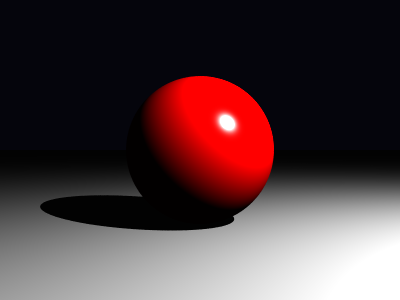
\includegraphics[width=\columnwidth]{../outputs/main_scene_20260405_190325/render.png}
\caption{Cena mínima com \texttt{PointLight}.}
\label{fig:main-scene}
\end{figure}

\subsection{Penumbra por fonte extensa}
\label{sec:experimentos-penumbra}

Arquivo âncora: \path{src/ray_tracing_2/main_area_light.py} (\texttt{render()}, l. 23; criação da \texttt{AreaLight}, l. 47-48).

Ao substituir a fonte pontual por uma fonte retangular amostrada, a borda de sombra deixa de ser descontínua e passa a ocupar uma região de penumbra. Esta imagem confirma empiricamente a leitura teórica sobre luz de área~\slidescite{inf2608slides05}{14--23}: a luz de área é uma integral sobre um emissor estendido aproximada por soma finita de amostras.

\begin{figure}[!ht]
\centering
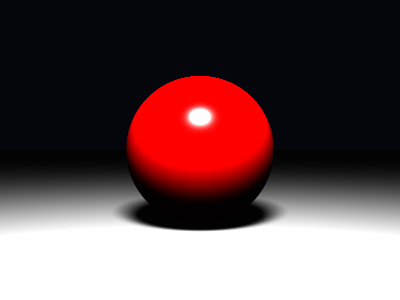
\includegraphics[width=\columnwidth]{../outputs/main_area_light_20260405_204336/render.png}
\caption{Penumbra com \texttt{AreaLight}.}
\label{fig:area-light}
\end{figure}

\subsection{Caixa tipo Cornell e instâncias geométricas}
\label{sec:experimentos-cornell-box}

Arquivo âncora: \path{src/ray_tracing_2/main_box.py} (\texttt{render()}, l. 63; paredes, l. 116; blocos instanciados, l. 140; luz pontual, l. 143).

Esta cena é importante menos pelo efeito óptico avançado e mais pela infraestrutura geométrica: cinco paredes, dois blocos instanciados e uma configuração fechada que expõe erros de transformação, orientação de normal e auto-interseção. Ela demonstra que \texttt{Instance} permite reusar caixas canônicas como blocos orientados e transladados sem reescrever a matemática de interseção.

\begin{figure}[!ht]
\centering
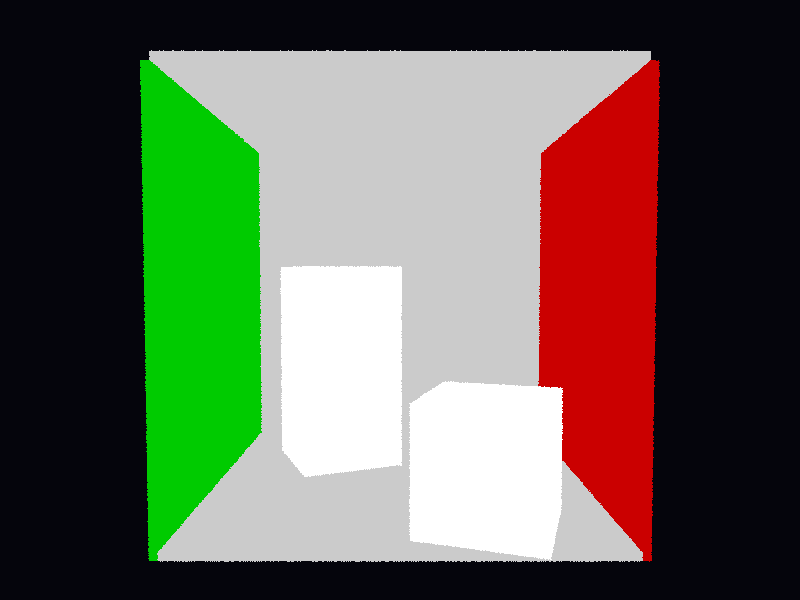
\includegraphics[width=\columnwidth]{../outputs/main_box_20260412_162658/render.png}
\caption{Cena tipo Cornell Box.}
\label{fig:main-box}
\end{figure}

\subsection{Malha triangular com BVH local}
\label{sec:experimentos-bvh-local}

Arquivo âncora: \path{src/ray_tracing_2/main_triangles.py} (\texttt{\_triangle\_mesh\_from\_spec()}, l. 39; \texttt{TriangleMesh.from\_vertices\_faces()}, l. 68; \texttt{render()}, l. 100; luzes, l. 179).

Esta é a evidência experimental mais importante para a parte de triângulos e aceleração~\slidescite{inf2608slides06}{3--36}. O arquivo \path{outputs/main_triangles_20260424_233034/properties.md} registra 5 vértices, 6 faces trianguladas, acelerador \texttt{bvh}, \texttt{bvh\_leaf\_size = 2}, 7 nós, 4 folhas e profundidade máxima 3. Portanto, o artigo pode afirmar com segurança que a malha triangular e a BVH local estão de fato ativas na renderização dessa cena específica.

\begin{figure}[!ht]
\centering
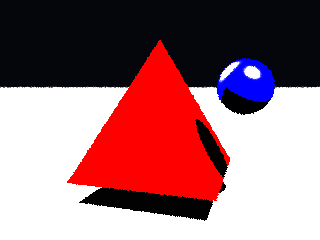
\includegraphics[width=\columnwidth]{../outputs/main_triangles_20260424_233034/render.png}
\caption{Malha triangular com BVH local.}
\label{fig:triangles-bvh}
\end{figure}

\subsection{Cornell Box com pirâmides refletiva e transparente}
\label{sec:experimentos-pyramids}

Arquivo âncora: \path{src/ray_tracing_2/cornell_box_pyramid.py} (\texttt{render()}, l. 50; construção das duas \texttt{TriangleMesh}, l. 167 e l. 174; luzes, l. 205 e l. 224).

Esta cena combina os dois eixos mais avançados do projeto: materiais recursivos~\slidescite{inf2608slides05}{26--35} e geometria triangulada~\slidescite{inf2608slides06}{3--14}. O arquivo \path{outputs/cornell_box_pyramid_20260425_003203/properties.md} confirma a presença de duas malhas triangulares distintas, uma transparente e outra refletiva, embutidas em uma cena fechada com múltiplas luzes. Isso a torna a melhor demonstração integrada de que triângulos, reflexão e refração não são módulos isolados, mas participam do mesmo pipeline de visibilidade e transporte local e recursivo.

\begin{figure}[!ht]
\centering
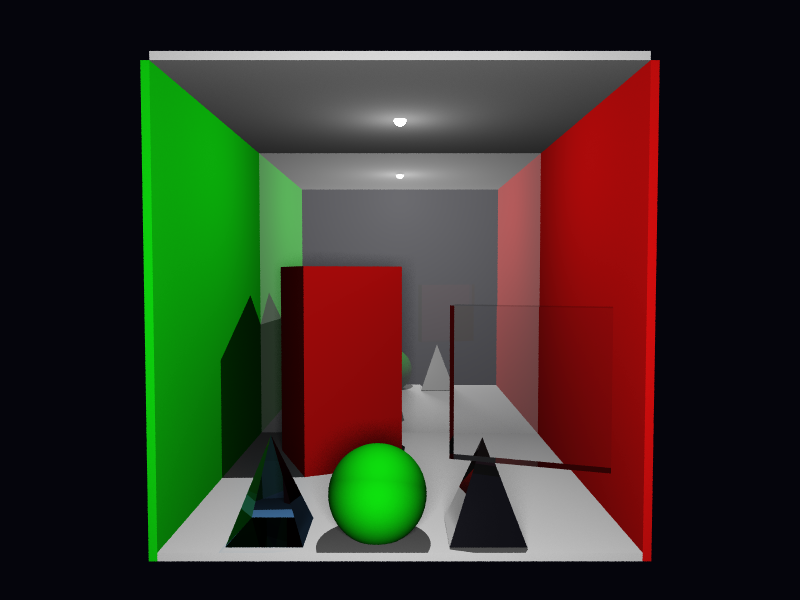
\includegraphics[width=\columnwidth]{../outputs/cornell_box_pyramid_20260425_003203/render.png}
\caption{Cornell Box com duas pirâmides trianguladas.}
\label{fig:pyramids-base}
\end{figure}

Uma execução mais recente da mesma cena, agora com \texttt{--spp 10} e \texttt{--sampling\_mode stratified}, reforça o mesmo ponto com uma evidência visual menos ruidosa e também documenta melhor o custo computacional da integração recursiva nessa configuração. O arquivo \path{outputs/cornell_box_pyramid_20260501_210143/properties.md} registra \texttt{samples\_per\_pixel = 10}, \texttt{sampling\_mode = stratified}, \texttt{render\_time\_seconds = 1035.4509} e \texttt{render\_time\_minutes = 17.2575}, mantendo a mesma combinação central de duas \texttt{TriangleMesh}, uma transparente e outra refletiva, em uma Cornell Box com luz de área e luzes pontuais auxiliares.

\begin{figure}[!ht]
\centering
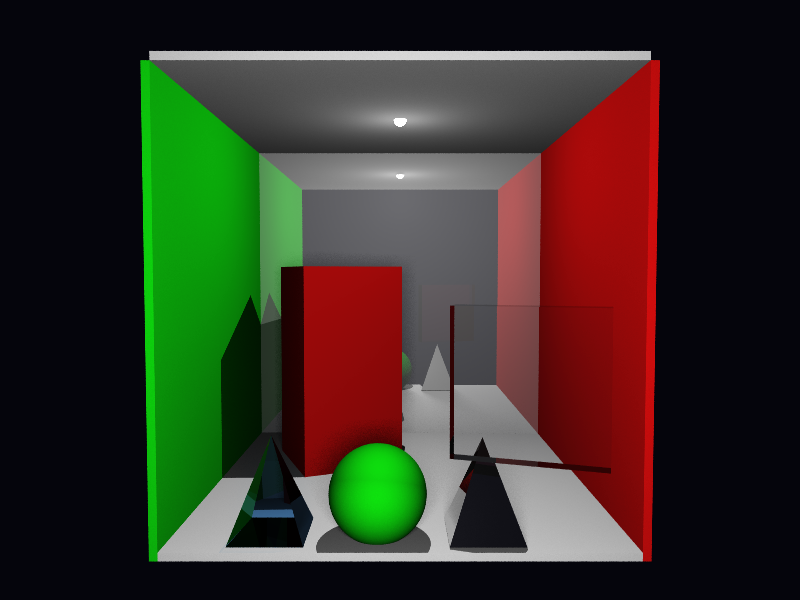
\includegraphics[width=\columnwidth]{../outputs/cornell_box_pyramid_20260501_210143/render.png}
\caption{Cornell Box com duas pirâmides trianguladas em spp 10 estratificado.}
\label{fig:pyramids-spp10}
\end{figure}

\subsection{Reprodutibilidade experimental por CLI padronizada}
\label{sec:experimentos-cli}

Embora a padronização do parser não altere a física do renderizador, ela melhora diretamente a rastreabilidade dos experimentos. Em particular, ela torna explícito um ponto conceitual importante do Slide 5: a amostragem bidimensional sobre o pixel~\slidescite{inf2608slides05}{4--9} e a amostragem bidimensional sobre a fonte extensa~\slidescite{inf2608slides05}{14--23} não são a mesma integral, ainda que ambas usem padrões 2D. Por isso, o repositório preserva dois controles públicos distintos, \texttt{sampling\_mode} para o filme e \texttt{light\_sampling\_mode} para \texttt{AreaLight}, enquanto reutiliza apenas uma infraestrutura interna compartilhada de geração de padrões 2D.

Do ponto de vista metodológico, essa separação é desejável: ela permite variar o estimador de anti-aliasing sem alterar a quadratura usada na integração da luz de área, e vice-versa. Isso reduz ambiguidade na interpretação dos resultados e melhora a comparabilidade entre execuções documentadas no próprio \texttt{properties.md}.

Exemplos mínimos de reprodução, todos com \texttt{800$\times$600} e \texttt{spp = 1}:

\begin{quote}
\small\ttfamily
python -m ray\_tracing\_2.main --width 800 --height 600 --spp 1\\
python -m ray\_tracing\_2.main\_area\_light --width 800 --height 600 --spp 1\\
\hspace*{1em}--sampling\_mode stratified --light\_sampling\_mode regular\\
python -m ray\_tracing\_2.cornell\_box --width 800 --height 600 --spp 1\\
\hspace*{1em}--sampling\_mode jittered --light\_sampling\_mode uniform\\
python -m ray\_tracing\_2.main\_triangles --width 800 --height 600 --spp 1\\
\hspace*{1em}--scene inputs/triangle\_pyramid.json --accelerator bvh\\
python -m ray\_tracing\_2.generate\_scene --input inputs/example\_scene.json\\
\hspace*{1em}--width 800 --height 600 --spp 1
\end{quote}

\traceability{\path{src/ray_tracing_2/cli.py} (\texttt{build\_parser()}, l. 14; \texttt{add\_sampling\_arguments()}, l. 37; \texttt{add\_light\_sampling\_argument()}, l. 52), \path{src/ray_tracing_2/sampling.py} (\texttt{uniform\_samples\_2d()}, l. 15; \texttt{regular\_grid\_samples\_2d()}, l. 26; \texttt{stratified\_grid\_samples\_2d()}, l. 42), \path{src/ray_tracing_2/film.py} (\texttt{SamplingMode}, l. 17; \texttt{get\_samples\_for\_pixel()}, l. 61), \path{src/ray_tracing_2/light.py} (\texttt{AreaLightSamplingMode}, l. 45; \texttt{\_iter\_sample\_uvs()}, l. 114; \texttt{sample\_radiance()}, l. 133), \path{src/ray_tracing_2/main.py} (\texttt{build\_cli\_parser()}, l. 79), \path{src/ray_tracing_2/main_area_light.py} (\texttt{build\_cli\_parser()}, l. 89), \path{src/ray_tracing_2/main_triangles.py} (\texttt{build\_cli\_parser()}, l. 202) e \path{src/ray_tracing_2/generate_scene.py} (\texttt{build\_cli\_parser()}, l. 122).}

\section{Limitações Atuais e Delimitação de Escopo}
\label{sec:limitacoes}

\subsection{Estruturas de aceleração ausentes ou apenas parciais}
\label{sec:limitacoes-aceleracao}

À luz do Slide 6~\citep{inf2608slides06}, a implementação atual cobre apenas uma fração do espaço de técnicas apresentado nos slides. O repositório não implementa grade regular, refinamento por SAT nem percorrimento incremental célula a célula~\slidescite{inf2608slides06}{15--21}; tampouco implementa SAH, compactação linear da BVH ou um agregador global de cena~\slidescite{inf2608slides06}{22--36}. O que existe de fato é uma BVH estática local a cada \texttt{TriangleMesh}, suficiente para reduzir o custo interno da malha, mas insuficiente para substituir uma estrutura de aceleração global do ray tracer.

Essa distinção é importante porque o custo no topo da cena continua linear. \texttt{Scene.compute\_intersection()} percorre \texttt{self.objects} de forma sequencial, de modo que a aceleração atua apenas dentro da malha triangulada, não entre esferas, caixas, instâncias e múltiplas malhas coexistindo na mesma cena. Portanto, a formulação correta no relatório não é ``o Slide 6 foi implementado'', mas sim ``parte do Slide 6 foi materializada por uma BVH local simplificada''.

\traceability{\path{src/ray_tracing_2/scene.py} (\texttt{compute\_intersection()}, l. 24), \path{src/ray_tracing_2/triangle_bvh.py} (\texttt{TriangleBVH}, l. 140; \texttt{\_build()}, l. 154; \texttt{TriangleBVHNode.intersect()}, l. 109).}

\subsection{Câmera e formação de imagem}
\label{sec:limitacoes-camera}

O projeto permanece estritamente no modelo pinhole apresentado no material introdutório sobre câmera~\slidescite{inf2608slides04}{19--39}. Isso significa que \texttt{Camera.generate\_ray()} sempre emite raios a partir de um único centro ótico, sem abertura finita, sem lente fina e sem profundidade de campo. A variável \texttt{focal\_distance} controla apenas a escala geométrica do plano de projeção, e não um mecanismo de focalização seletiva.

Essa limitação não invalida o modelo adotado; ela apenas delimita seu alcance. O supersampling discutido no bloco de amostragem~\slidescite{inf2608slides05}{4--8} melhora a aproximação da média radiância por pixel, mas não altera a física óptica da câmera. Logo, qualquer leitura do resultado visual deve ser feita como imagem de câmera pinhole com amostragem estocástica, e não como imagem com desfoque óptico de lente.

\traceability{\path{src/ray_tracing_2/camera.py} (\texttt{Camera.\_\_init\_\_()}, l. 7; \texttt{generate\_ray()}, l. 23), \path{src/ray_tracing_2/film.py} (\texttt{get\_samples\_for\_pixel()}, l. 60).}

\subsection{Convenções radiométricas e simplificações de iluminação}
\label{sec:limitacoes-radiometria}

Há uma simplificação deliberada e potencialmente enganosa se não for declarada: \texttt{PointLight} e \texttt{AreaLight} não seguem a mesma convenção radiométrica nesta base. Os slides de iluminação pontual apresentam o decaimento geométrico clássico por $1/r^2$~\slidescite{inf2608slides04}{40--41}, mas \texttt{PointLight.radiance()} preserva a convenção do enunciado principal e trata \texttt{power} como radiância incidente constante modulada apenas por visibilidade e transmitância. Já \texttt{AreaLight.sample\_radiance()} distribui energia por amostras do emissor e introduz explicitamente o termo geométrico de distância.

O resultado prático é um subsistema de luzes internamente heterogêneo, embora coerente com os objetivos pedagógicos do projeto. Essa decisão é defensável para o Projeto 1, mas precisa ser descrita como simplificação de modelagem, e não como equivalência física entre fonte pontual ideal, emissor extenso e formulação radiométrica completa.

\traceability{\path{src/ray_tracing_2/light.py} (\texttt{PointLight.radiance()}, l. 46; \texttt{AreaLight.sample\_radiance()}, l. 92).}

\subsection{Materiais recursivos e truncamento computacional}
\label{sec:limitacoes-materiais}

Os materiais reflexivo e transparente representam uma extensão substancial do núcleo local de Phong, mas permanecem aproximativos sob o ponto de vista da física de materiais. \texttt{ReflectiveMaterial.eval()} mistura Phong local e reflexão recursiva com Fresnel-Schlick de maneira plausível, porém não equivalente a um BRDF fisicamente baseado. \texttt{TransparentMaterial.eval()} usa Snell, TIR e Beer-Lambert, mas assume meio homogêneo, atenuação por canal RGB e ausência de dispersão espectral contínua.

Além disso, toda a recursão é truncada por \texttt{max\_depth}. Isso é necessário para conter custo computacional e evitar crescimento exponencial do número de raios, mas significa que o traçador resolve apenas uma aproximação finita de cadeias longas de reflexão e transmissão. A leitura correta, portanto, é a de um ray tracer recursivo de profundidade limitada, não a de um solucionador completo de transporte de luz.

\traceability{\path{src/ray_tracing_2/material.py} (\texttt{ReflectiveMaterial.eval()}, l. 101; \texttt{TransparentMaterial.eval()}, l. 186; \texttt{TransparentMaterial.shadow\_transmittance()}, l. 167), \path{src/ray_tracing_2/scene.py} (\texttt{can\_spawn\_ray()}, l. 41).}

\subsection{Leitura correta frente ao enunciado principal}
\label{sec:limitacoes-escopo}

Frente a \path{materiais/proj1.pdf}, a interpretação tecnicamente correta é que o repositório cobre com segurança o núcleo exigido pelo projeto e ainda incorpora várias extensões relevantes da disciplina: supersampling, instanciação, luz de área, materiais recursivos, malha triangular e BVH local. Por outro lado, ele não esgota o espaço teórico apresentado nas aulas, sobretudo na parte de aceleração e na parte de modelagem física mais rigorosa da câmera, das fontes e dos materiais.

Essa delimitação é importante para o valor científico do artigo. O mérito do trabalho não está em inflar o escopo entregue, mas em mostrar com precisão onde a implementação coincide com a teoria ensinada, onde a simplifica e onde conscientemente para.

\section{Diagramas como Camada Adicional de Rastreabilidade}
\label{sec:experimentos-diagramas}

Além das imagens de saída das cenas, o repositório inclui diagramas PlantUML efetivamente renderizados em PNG, que funcionam como documentação intermediária entre o texto deste artigo e o código executável. O ponto metodológico importante é que esses diagramas não substituem a análise anterior; eles a condensam em vistas complementares do pipeline real, já validadas sintaticamente pelo próprio PlantUML.

Para evitar que quatro figuras largas interrompam a leitura do desenvolvimento principal, os diagramas foram deslocados para um anexo ao final do artigo. Essa mudança é apenas editorial: o papel analítico do conjunto permanece o mesmo.

O anexo reúne quatro vistas complementares. A Figura~\ref{fig:diagram-overview} sintetiza o fluxo entre entrypoint, \texttt{cli.py}, \texttt{CommonRenderOptions}, construção de cena e câmera, \texttt{Render.render()}, \texttt{Film.render()} e geração de \texttt{render.png}, \texttt{properties.json} e \texttt{properties.md}. A Figura~\ref{fig:diagram-trace} isola o trecho mais denso do material sobre reflexão, refração e transmitância, isto é, amostragem do filme, despacho por material, recursão por profundidade, reflexão, refração e transmitância em raios de sombra. A Figura~\ref{fig:diagram-bvh} deixa explícito que a poda por AABB e a travessia da BVH acontecem dentro de \texttt{TriangleMesh}, e não como acelerador global da cena, enquanto a Figura~\ref{fig:diagram-class} complementa as vistas dinâmicas com uma visão estrutural estática das principais dependências do pacote.

Em conjunto, esses artefatos visuais fortalecem a rastreabilidade do artigo: as Seções~\ref{sec:slide4} e~\ref{sec:slide5} ganham uma representação operacional do pipeline completo, enquanto a Seção~\ref{sec:slide6} passa a contar com uma visualização explícita da fronteira entre interseção global da cena e aceleração local de malhas triangulares.

\section{Conclusão, Avaliação Final e Disponibilidade de Artefatos}
\label{sec:conclusao}

O Projeto 1 implementa de forma sólida o núcleo geométrico e fotométrico do traçador e a maior parte das extensões ópticas e amostrais discutidas ao longo do artigo. O resultado é um ray tracer com câmera pinhole, interseções analíticas, Phong local, sombras duras, supersampling, instanciação, luz de área, reflexão com Fresnel-Schlick, refração dielétrica com Snell e TIR, além de atenuação Beer-Lambert em raios refratados e de sombra.

O principal cuidado técnico desta versão é deixar claro o estatuto da geometria triangular e da aceleração frente às limitações consolidadas na Seção~\ref{sec:limitacoes}. O repositório entrega triangulação, \texttt{TriangleMesh} e uma BVH estática local construída por mediana no eixo dominante, com poda por AABB e travessia ordenada aproximadamente pela entrada do raio. Isso é suficiente para caracterizar uma aceleração real da malha, mas não autoriza afirmar implementação de grade regular, SAH, BVH linearizada ou agregador global de cena.

 Tomando o estado atual do repositório como objeto de avaliação, a implementação entrega de forma efetiva um \emph{ray tracer} educacional reprodutível, com núcleo geométrico-fotométrico completo, várias extensões relevantes do material da disciplina e uma camada operacional de execução suficientemente organizada para experimentação controlada. Em particular, o projeto já não deve ser lido apenas como um conjunto de cenas isoladas: ele possui um núcleo comum de CLI, uma convenção relativamente estável de geração de artefatos e uma fronteira explícita entre o que está fisicamente simplificado e o que está de fato operacionalizado no código. Os quadros consolidados reunidos no anexo final organizam essa leitura em três tabelas: a Tabela~\ref{tab:slide4-aderencia} sintetiza os conteúdos do Slide 4, a Tabela~\ref{tab:slide5-aderencia} resume os conteúdos do Slide 5 e a Tabela~\ref{tab:slide6-aderencia} reúne o bloco de triângulos e estruturas de aceleração correspondente ao Slide 6.

Sob o critério do Projeto 1, essa entrega é tecnicamente robusta e supera o núcleo mínimo ao incorporar supersampling, luz de área, materiais recursivos, geometria triangular e aceleração local por BVH. Sob o critério mais forte de cobertura integral do arco teórico das aulas, a entrega permanece conscientemente parcial. Essa parcialidade, contudo, não é caótica: ela é bem localizada. O que falta está concentrado em modelagem física mais rigorosa e em estruturas de aceleração mais sofisticadas, e não em inconsistência do pipeline principal.

Há também um ponto metodológico importante: a implementação agora entrega não apenas imagens, mas também rastreabilidade experimental. A combinação entre \path{src/ray_tracing_2/cli.py}, \path{src/ray_tracing_2/render.py} e \path{src/ray_tracing_2/render_snapshot.py} faz com que cada execução relevante preserve resolução, modo de amostragem, semente, tempo de render e descrição estruturada da cena em artefatos persistentes. Isso aumenta o valor científico do projeto porque permite distinguir claramente entre efeito visual observado, parâmetro de entrada e hipótese geométrica ou física codificada.

Os artefatos de pesquisa discutidos neste artigo estão disponíveis no repositório do projeto~\citep{inf2608projectrepo}. Em particular, o código-fonte analisado permanece versionado em \path{src/}, as cenas de entrada em \path{inputs/}, as renderizações e seus metadados persistidos em \path{outputs/} e os diagramas utilizados nesta discussão foram mantidos em formato renderizado junto ao repositório. Essa organização torna reprodutíveis tanto os resultados visuais quanto os parâmetros de execução usados na avaliação final.

\traceability{\path{src/ray_tracing_2/cli.py} (\texttt{CommonRenderOptions}; \texttt{add\_common\_render\_arguments()}), \path{src/ray_tracing_2/film.py} (\texttt{SamplingMode}; \texttt{get\_samples\_for\_pixel()}), \path{src/ray_tracing_2/light.py} (\texttt{AreaLight}; \texttt{AreaLightSamplingMode}; \texttt{sample\_radiance()}), \path{src/ray_tracing_2/render.py} (\texttt{Render.render()}), \path{src/ray_tracing_2/render_snapshot.py} (\texttt{RenderSnapshot.from\_runtime()}; \texttt{to\_markdown()}), \path{src/ray_tracing_2/shape.py} (\texttt{Triangle}; \texttt{TriangleMesh}; \texttt{Instance}), \path{src/ray_tracing_2/triangle_bvh.py} (\texttt{AABB}; \texttt{TriangleBVH}).}

\section{Quadros Consolidados de Aderência entre Referência e Implementação}
\label{sec:quadros-aderencia}

Esta seção reúne, em formato sintético, a leitura dos quadros de aderência deslocados das seções analíticas anteriores. Eles devem ser lidos como consolidação comparativa do que já foi discutido no corpo do artigo, em articulação com os slides da disciplina e com as referências selecionadas de \pbrtbook.

Para evitar que três tabelas largas quebrem o fechamento do argumento principal, os quadros consolidados foram deslocados para um anexo ao final do artigo. O que permanece aqui é a chave de leitura de cada quadro, isto é, o enquadramento interpretativo necessário para que as tabelas sejam lidas como síntese comparativa, e não como inventário isolado.

\subsection{Núcleo geométrico e fotométrico}

O Quadro~\ref{tab:slide4-aderencia} deve ser lido como a síntese do bloco mais estável e mais completamente materializado do repositório. Ele mostra que a cadeia câmera-raio-hit-sombreamento está operacional de ponta a ponta, ao mesmo tempo em que explicita duas qualificações importantes para a leitura técnica desta entrega: a convenção simplificada adotada para \texttt{PointLight} e a presença, já nesse núcleo, de um teste de sombra implementado em forma mais geral por transmitância acumulada.

\subsection{Extensões ópticas e amostrais}

O Quadro~\ref{tab:slide5-aderencia} consolida o trecho em que a implementação mais se afasta do núcleo mínimo e passa a operar por aproximações controladas. A leitura correta não é a de um bloco fisicamente completo, mas a de um conjunto coerente de extensões efetivas: amostragem estocástica do pixel, instanciação afim, integração discreta sobre luz de área, reflexão com Fresnel-Schlick, refração com Snell e Beer-Lambert, além da separação metodologicamente útil entre \texttt{sampling\_mode} no filme e \texttt{light\_sampling\_mode} na fonte extensa.

\subsection{Geometria triangular e estruturas de aceleração}

O Quadro~\ref{tab:slide6-aderencia} precisa ser interpretado com mais cuidado do que os anteriores porque o Slide 6 combina, no mesmo arco didático, conteúdo realmente entregue e conteúdo apenas parcialmente coberto. A evidência positiva está em \texttt{Triangle}, \texttt{TriangleMesh}, AABB e BVH local por malha; a evidência negativa é igualmente importante: o repositório não implementa grade regular, SAH, BVH linearizada nem agregador global de cena. O valor deste quadro está justamente em impedir uma leitura inflada da cobertura do bloco de aceleração.

\begin{declarations}

\begin{contributions}
Yang Ricardo Barcellos Miranda foi responsável pela organização do manuscrito, consolidação da análise técnico-científica do repositório, revisão do alinhamento entre slides, PBRT e implementação, e preparação da versão atual em \LaTeX.
\end{contributions}

\begin{aitools}
Ferramentas de IA generativa foram utilizadas como apoio à revisão textual, reorganização do conteúdo técnico e padronização da redação em \LaTeX. Todo o conteúdo técnico final foi revisado e validado pelo autor.
\end{aitools}

\end{declarations}

\bibliographystyle{apalike-sol}
\bibliography{refs}

\clearpage
\section*{Anexo: Quadros Consolidados de Aderência}

Os quadros desta seção final reúnem, em formato tabular, a síntese comparativa discutida na Seção~\ref{sec:quadros-aderencia}. Eles foram deslocados para o anexo para preservar a continuidade da leitura analítica e do fechamento do artigo.

\subsection*{Núcleo geométrico e fotométrico}

\begin{table*}[!ht]
\caption{Quadro consolidado de aderência entre os conteúdos do Slide 4 e a implementação atual.}
\label{tab:slide4-aderencia}
\centering
\begin{tblr}{
width=\textwidth,
colspec={Q[l,wd=0.24\textwidth] Q[l,wd=0.17\textwidth] Q[l,wd=0.50\textwidth]},
row{1}={font=\bfseries},
rows={valign=t}
}
Conceito de referência & Situação no repositório & Evidência \\
Raio paramétrico e registro de hit & Implementado & \texttt{Ray}; \texttt{Hit}; \texttt{Scene.compute\_intersection()} \\
Interseção raio-plano & Implementado & \texttt{Plane.intersect()} \\
Interseção raio-esfera & Implementado & \texttt{Sphere.intersect()} \\
Tolerância numérica para evitar auto-interseção & Implementado & \texttt{Scene.offset\_point()}; limiar positivo nas interseções \\
Câmera pinhole e geração de raios primários & Implementado & \texttt{Camera.\_\_init\_\_()}; \texttt{Camera.generate\_ray()} \\
Mudança de base entre espaço da câmera e espaço global & Implementado & \texttt{glm.lookAt()} + \texttt{inv\_view} em \texttt{Camera} \\
Modelo local de Phong com ambiente, difusa e especular & Implementado & \texttt{PhongMaterial.direct\_lighting()}; \texttt{PhongMaterial.eval()} \\
Sombra dura por teste de visibilidade & Implementado com generalização & \texttt{Scene.transmittance()} reduz-se ao caso binário para opacos e estende o slide para transparentes \\
Luz pontual com síntese radiométrica do slide & Implementado com simplificação & \texttt{PointLight.radiance()} usa a convenção do enunciado sem queda explícita por $1/r^2$ \\
Estrutura algorítmica básica câmera-hit-sombreamento & Implementado & \texttt{Film.render()}; \texttt{Camera.generate\_ray()}; \texttt{Scene.trace\_ray()} \\
\end{tblr}
\end{table*}

\subsection*{Extensões ópticas e amostrais}

\begin{table*}[!ht]
\caption{Quadro consolidado de aderência entre os conteúdos do Slide 5 e a implementação atual.}
\label{tab:slide5-aderencia}
\centering
\begin{tblr}{
width=\textwidth,
colspec={Q[l,wd=0.25\textwidth] Q[l,wd=0.17\textwidth] Q[l,wd=0.50\textwidth]},
row{1}={font=\bfseries},
rows={valign=t}
}
Conceito de referência & Situação no repositório & Evidência \\
Antialiasing por múltiplas amostras por pixel & Implementado com extensão & \texttt{sampling.uniform\_samples\_2d()}; \texttt{sampling.stratified\_grid\_samples\_2d()}; \texttt{Film.get\_samples\_for\_pixel()}; \texttt{Film.render()} \\
Jitter subpixel aleatório & Implementado & \texttt{SamplingMode.JITTERED}; \texttt{sampling.uniform\_samples\_2d()}; \texttt{Film.get\_samples\_for\_pixel()} \\
Amostragem estratificada & Implementado como extensão & \texttt{SamplingMode.STRATIFIED}; \texttt{sampling.stratified\_grid\_samples\_2d()}; \texttt{Film.get\_samples\_for\_pixel()} \\
Instanciação por transformações afins em coordenadas homogêneas & Implementado & \texttt{Instance.intersect()}; \texttt{main\_ellipse.py}; \texttt{main\_box.py} \\
Transformação correta de normais por inversa transposta & Implementado & \texttt{m\_inv\_t} em \texttt{Instance.intersect()} \\
Luz de área com integração discreta e penumbra & Implementado com aproximação & \texttt{AreaLight.sample\_radiance()}; \texttt{AreaLight.radiance()}; \texttt{main\_area\_light.py} \\
Padrões regular e uniforme puros para amostragem da luz & Implementado com modos explícitos & \texttt{AreaLightSamplingMode.REGULAR}; \texttt{AreaLightSamplingMode.UNIFORM}; \texttt{sampling.regular\_grid\_samples\_2d()}; \texttt{sampling.uniform\_samples\_2d()}; \texttt{AreaLight.\_iter\_sample\_uvs()} \\
Caixa/AABB e método de slabs & Implementado & \texttt{Box.intersect()}; \texttt{AABB.intersects()} \\
Traçador recursivo com profundidade finita & Implementado & \texttt{Scene.can\_spawn\_ray()}; \texttt{Scene.trace\_ray()} \\
Reflexão especular com Fresnel-Schlick & Implementado com aproximação & \texttt{ReflectiveMaterial.eval()} \\
Refração dielétrica com Snell, TIR e Beer-Lambert & Implementado com simplificação & \texttt{TransparentMaterial.eval()}; \texttt{TransparentMaterial.shadow\_transmittance()} \\
Generalização do shadow ray para transmitância acumulada & Implementado & \texttt{Scene.transmittance()} \\
\end{tblr}
\end{table*}

\subsection*{Geometria triangular e estruturas de aceleração}

\begin{table*}[!ht]
\caption{Quadro consolidado de aderência entre os conteúdos do Slide 6 e a implementação atual.}
\label{tab:slide6-aderencia}
\centering
\begin{tblr}{
width=\textwidth,
colspec={Q[l,wd=0.25\textwidth] Q[l,wd=0.17\textwidth] Q[l,wd=0.50\textwidth]},
row{1}={font=\bfseries},
rows={valign=t}
}
Conceito de referência & Situação no repositório & Evidência \\
Triângulo como primitiva elementar & Implementado & \texttt{Triangle}; vetores de aresta \texttt{e1}/\texttt{e2}; normal geométrica \\
Interseção raio-triângulo por Möller-Trumbore & Implementado & \texttt{Triangle.intersect()} \\
Malha triangulada por vértices e faces & Implementado & \texttt{TriangleMesh}; \texttt{TriangleMesh.from\_vertices\_faces()} \\
Integração da malha ao pipeline geral da cena & Implementado & \texttt{Scene.compute\_intersection()}; \texttt{main\_triangles.py}; \texttt{Instance.intersect()} \\
BVH local para malhas triangulares & Implementado com simplificação & \texttt{TriangleBVH}; \texttt{TriangleBVHNode.intersect()}; constru{\c c}{\~a}o por mediana no eixo dominante \\
Caixas AABB como volumes de contenção & Implementado & \texttt{AABB}; \texttt{AABB.intersects()} \\
Travessia recursiva com poda local por malha & Implementado com simplificação & ordem aproximada pela entrada do raio em \texttt{TriangleBVHNode.intersect()} \\
Grade regular para aceleração global & Não implementado & ausente no repositório; a cena continua sem grade uniforme global \\
SAH, BVH linearizada e agregador global de cena & Não implementado & \texttt{Scene.compute\_intersection()} permanece sequencial; não há SAH nem estrutura global de aceleração \\
\end{tblr}
\end{table*}

\clearpage
\section*{Anexo: Diagramas de Rastreabilidade}

Para preservar a fluidez do corpo principal, os diagramas discutidos na Seção~\ref{sec:experimentos-diagramas} foram reunidos neste anexo final. Eles mantêm a mesma função metodológica: servir como ponte entre a formulação textual do artigo e a organização efetiva do código executável.

\subsection*{Visão geral do pipeline}

Este diagrama sintetiza o fluxo entre entrypoint, \texttt{cli.py}, \texttt{CommonRenderOptions}, construção de cena e câmera, \texttt{Render.render()}, \texttt{Film.render()} e geração de \texttt{render.png}, \texttt{properties.json} e \texttt{properties.md}.

\begin{figure*}[!ht]
\centering
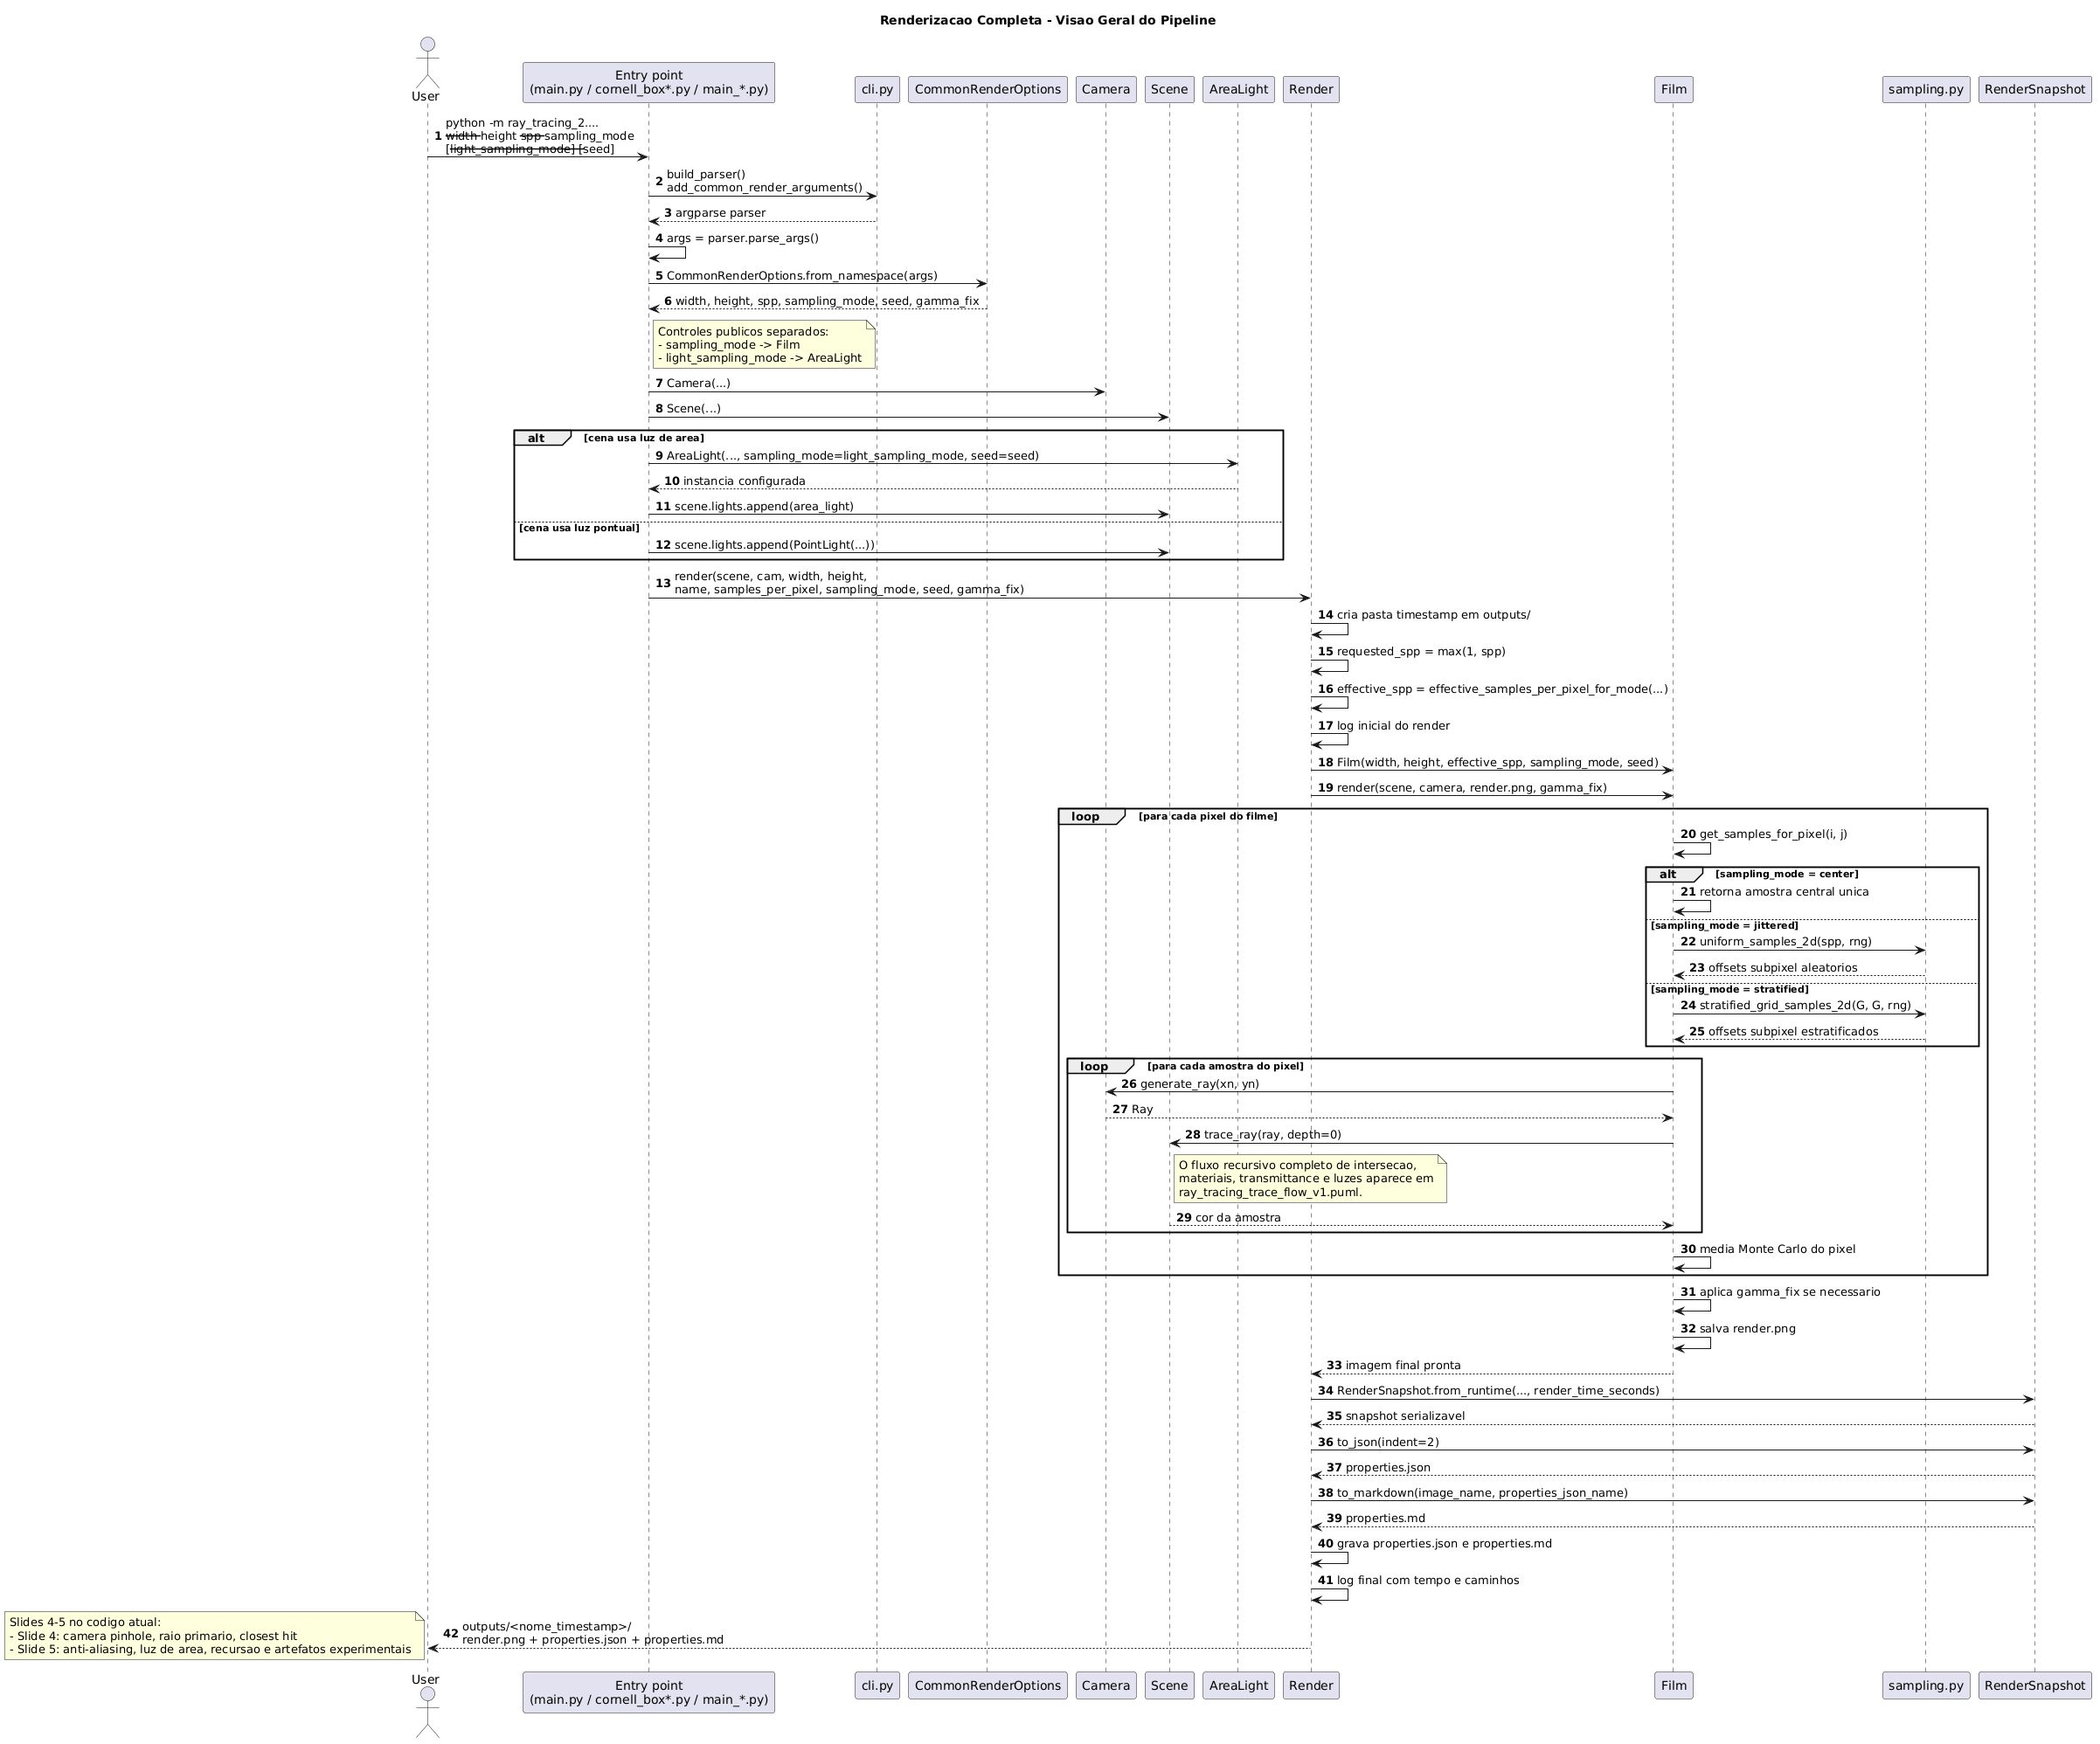
\includegraphics[width=0.95\textwidth]{../ray_tracing_render_overview_v1.puml.png}
\caption{Diagrama renderizado da visão geral do pipeline.}
\label{fig:diagram-overview}
\end{figure*}

\subsection*{Fluxo dinâmico de sombreamento recursivo}

Esta vista separa do overview o trecho mais denso do material sobre reflexão, refração e transmitância, isto é, amostragem do filme, despacho por material, recursão por profundidade, reflexão, refração e transmitância em raios de sombra.

\begin{figure*}[!ht]
\centering
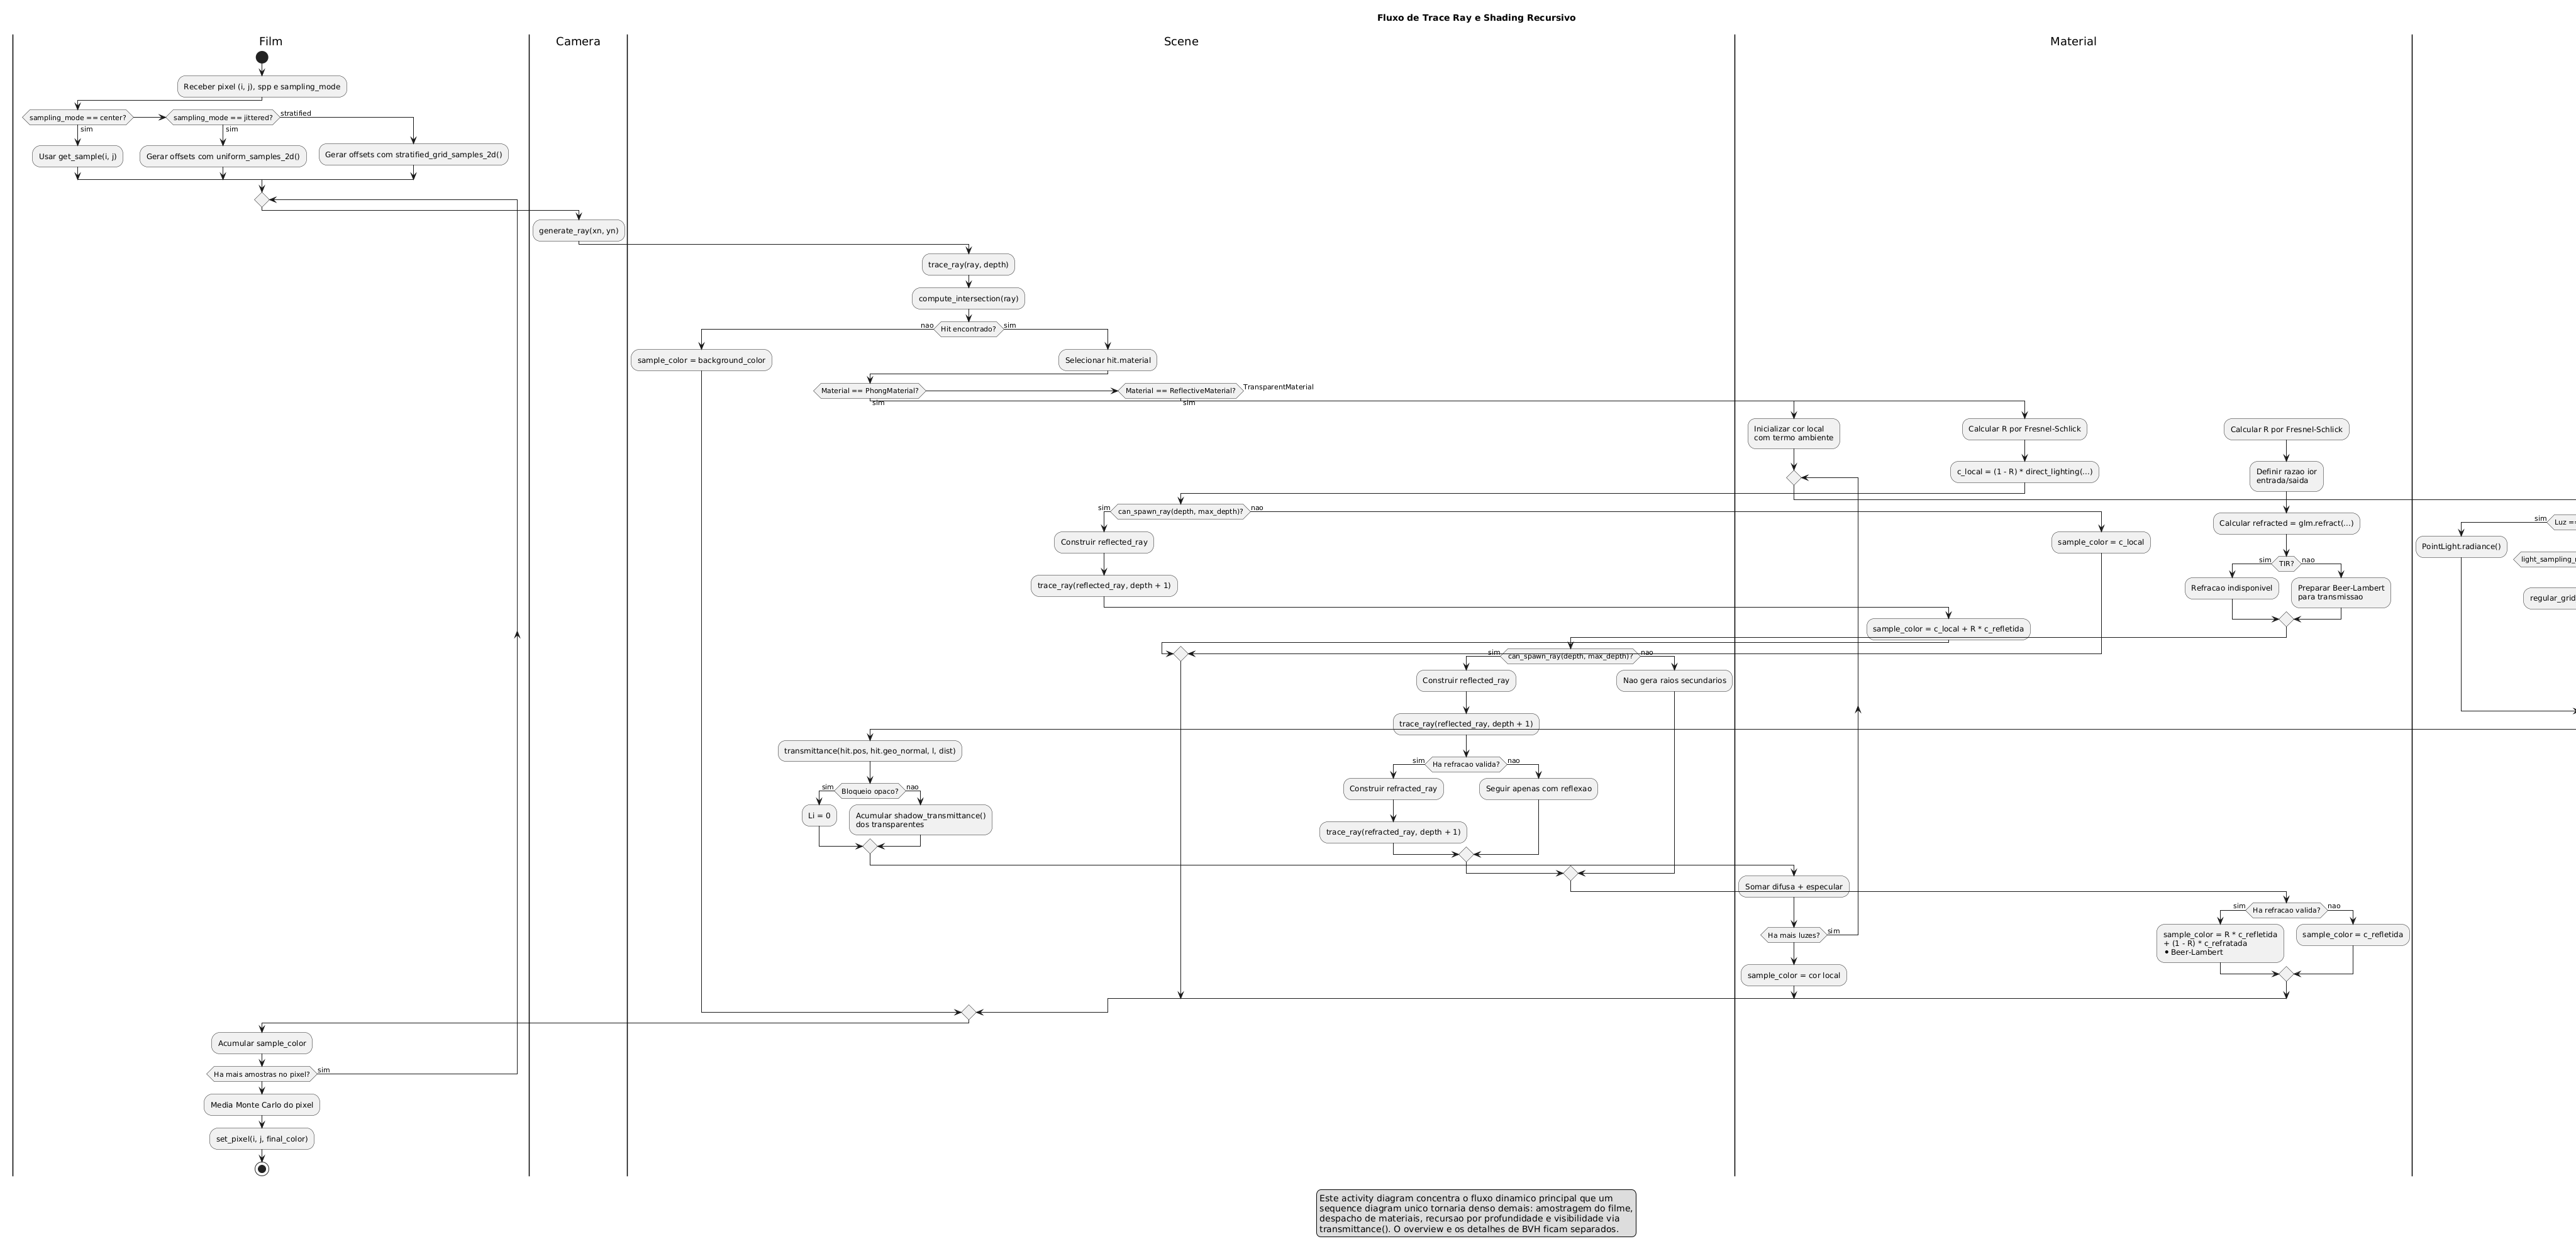
\includegraphics[width=0.95\textwidth]{../ray_tracing_trace_flow_v1.puml.png}
\caption{Diagrama renderizado do fluxo de \texttt{trace\_ray} e shading recursivo.}
\label{fig:diagram-trace}
\end{figure*}

\subsection*{Fluxo local de aceleração para malhas}

Este diagrama deixa explícito que a poda por AABB e a travessia da BVH acontecem dentro de \texttt{TriangleMesh}, e não como acelerador global da cena, o que reforça a leitura defendida na Seção~\ref{sec:slide6}.

\begin{figure*}[!ht]
\centering
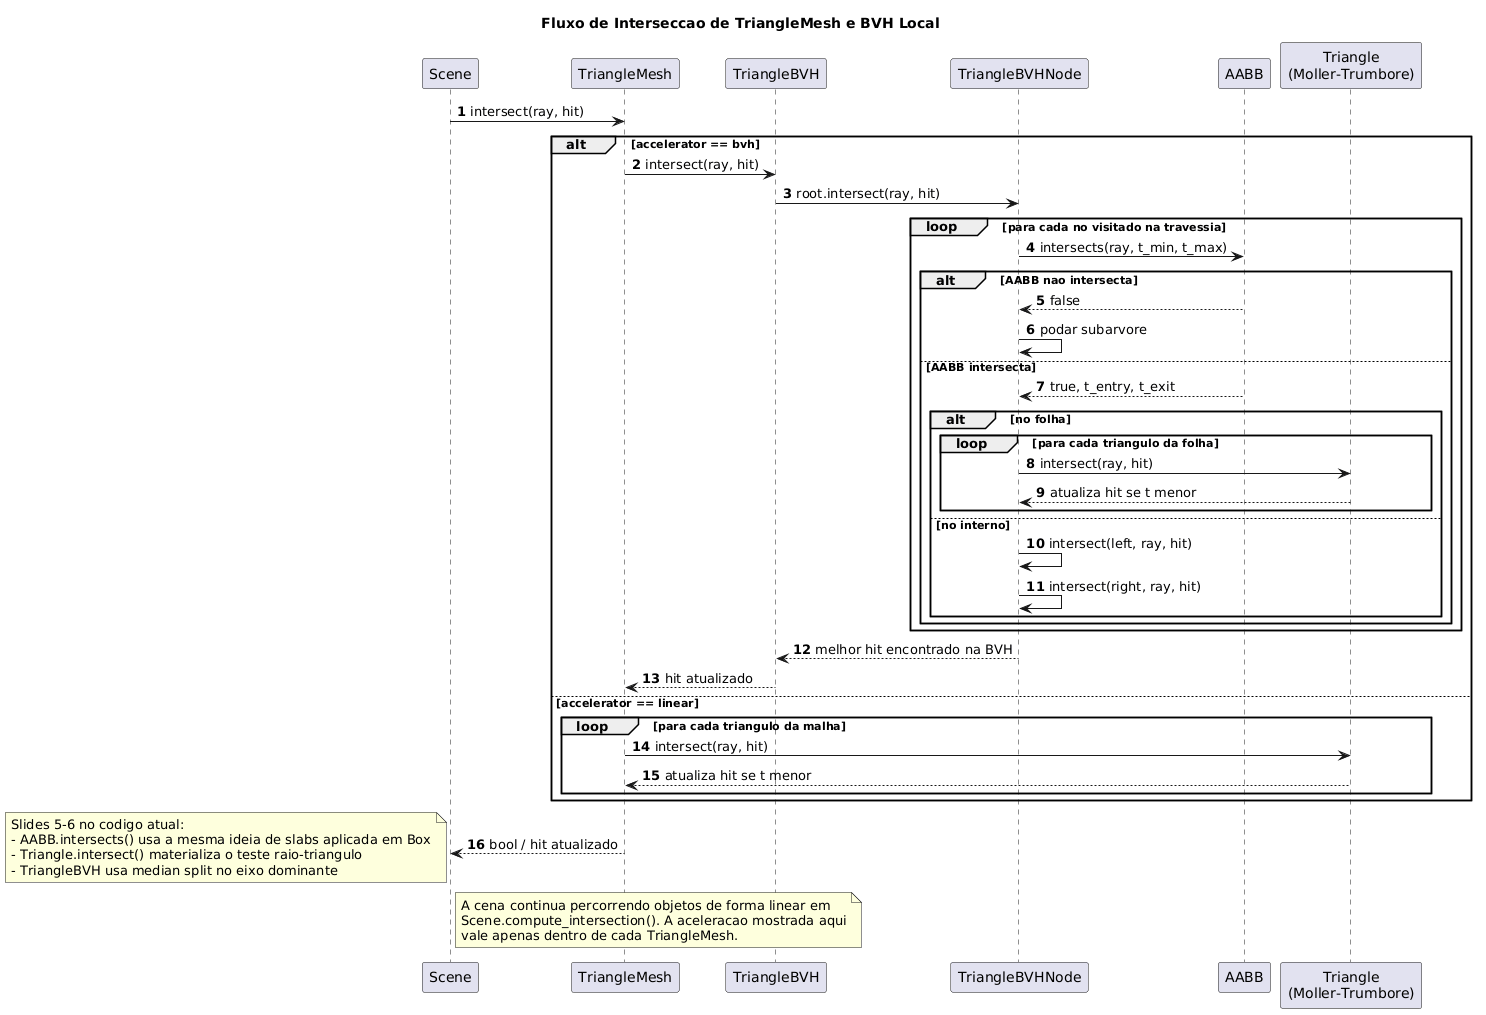
\includegraphics[width=0.95\textwidth]{../ray_tracing_bvh_flow_v1.puml.png}
\caption{Diagrama renderizado do fluxo local de BVH para \texttt{TriangleMesh}.}
\label{fig:diagram-bvh}
\end{figure*}

\subsection*{Visão estrutural estática}

Esta imagem complementa os diagramas dinâmicos ao mostrar dependências entre \texttt{Render}, \texttt{Scene}, \texttt{Film}, \texttt{Camera}, \texttt{Light}, \texttt{Material}, \texttt{TriangleMesh} e \texttt{TriangleBVH}.

\begin{figure*}[!ht]
\centering
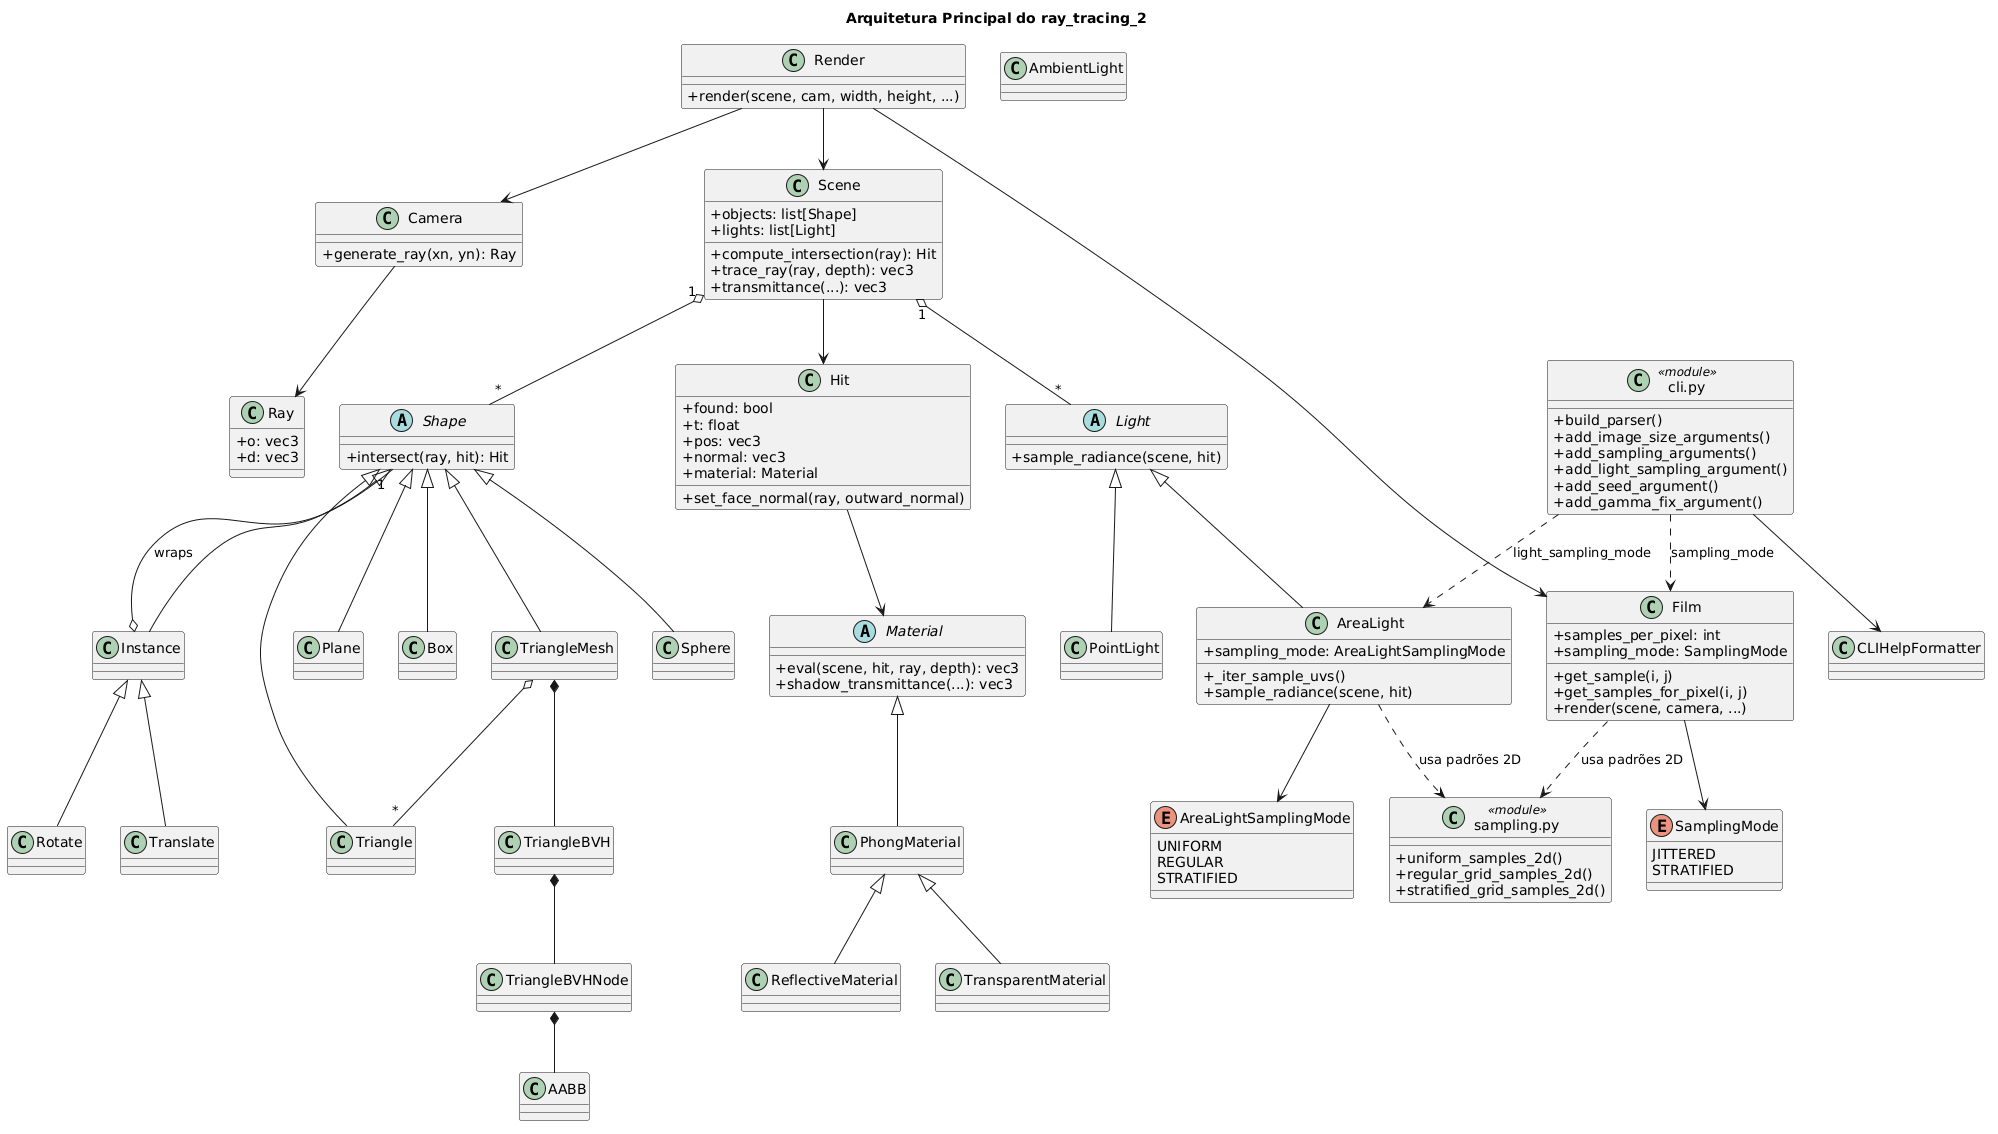
\includegraphics[width=0.95\textwidth]{../ray_tracing_2_class-diagram.puml.png}
\caption{Diagrama renderizado da arquitetura principal do \texttt{ray\_tracing\_2}.}
\label{fig:diagram-class}
\end{figure*}

\end{document}
